%! Author = leo
%! Date = 25.07.20

% Preamble
\documentclass{beamer}
\usetheme[subsectionpage=progressbar]{metropolis}
\usepackage[backend=bibtex,style=numeric]{biblatex}
\addbibresource{literature.bib}
\setbeamertemplate{bibliography item}{\insertbiblabel}

% Packages
\usepackage{amsmath}
\usepackage{amssymb}
\usepackage{bm}
\usepackage{adjustbox}
\usepackage{mathtools}
\usepackage{booktabs}
\usepackage{algorithm}
\usepackage{microtype}
\usepackage{algpseudocode}
\usepackage{subcaption}
\usepackage{tabularx}
\usepackage[normalem]{ulem}
\usepackage{graphicx}
\usepackage{appendixnumberbeamer}

\setcounter{tocdepth}{1}

% Commands
\DeclarePairedDelimiterX{\infdivx}[2]{(}{)}{%
#1\;\delimsize\|\;#2%
}
\newcommand{\kldiv}{D_{KL}\infdivx}

\makeatletter
\newenvironment{breakablealgorithm}
{% \begin{breakablealgorithm}
\begin{center}
\refstepcounter{algorithm}% New algorithm
    \vspace{1em}
    \hrule height.8pt depth0pt \kern2pt% \@fs@pre for \@fs@ruled
    \renewcommand{\caption}[2][\relax]{% Make a new \caption
    {\raggedright\textbf{\ALG@name~\thealgorithm} ##2\par}%
    \ifx\relax##1\relax % #1 is \relax
    \addcontentsline{loa}{algorithm}{\protect\numberline{\thealgorithm}##2}%
    \else % #1 is not \relax
    \addcontentsline{loa}{algorithm}{\protect\numberline{\thealgorithm}##1}%
    \fi
    \kern2pt\hrule\kern4pt
    }
}{% \end{breakablealgorithm}
\kern2pt\hrule\relax% \@fs@post for \@fs@ruled
\vspace{1em}
\end{center}
}
\makeatother
\title{Semantic Representations in Variational Autoencoders as a Model of the Visual System}
\subtitle{Master Thesis Presentation}
\author{Leonard Papenmeier}
\date{\today}

% Document
\begin{document}
\maketitle
\begin{frame}{Outline}
\tableofcontents
\end{frame}


\section{Introduction}
\begin{frame}{Biological Plausibility}
\begin{columns}
\begin{column}{0.48\textwidth}
Supervised CNNs have shown relatedness to the Visual System:
\begin{itemize}
\item Emergence of Gabor wavelets~\cite{krizhevsky2012imagenet}
\item Explanation of IT activity~\cite{khaligh2014deep}
\end{itemize}
\end{column}
\begin{column}{0.48\textwidth}
\begin{figure}
\centering
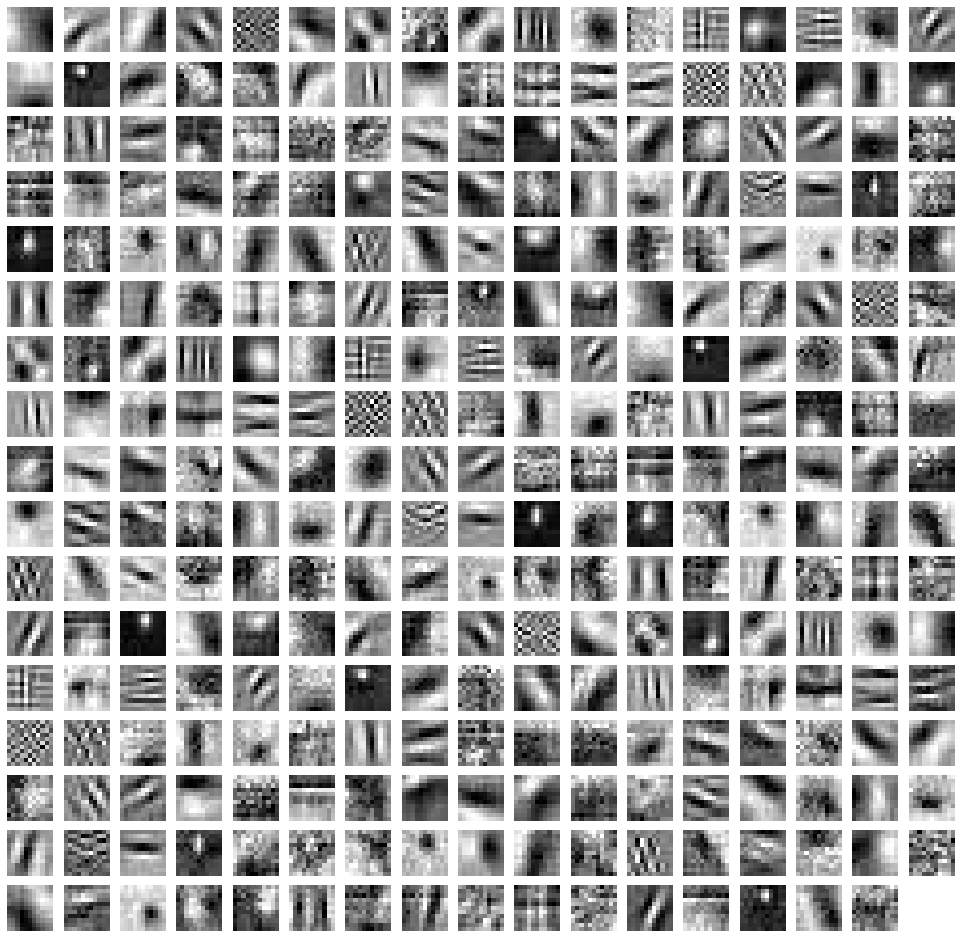
\includegraphics[width=\textwidth]{images/alexnet_classification_l1_kernels.png}
\caption{Gabor Wavelets in the first Layer of AlexNet~\cite{krizhevsky2012imagenet}}
\label{fig:figure_gabor}
\end{figure}
\end{column}
\end{columns}
\end{frame}
\begin{frame}{Variational Autoencoder (VAE)}
\begin{columns}
\begin{column}{0.48\textwidth}
\begin{itemize}
\item Requires no labeled data
\item Allows sampling of latent space
\item Topographic map
\item Latent space arithmetic
\end{itemize}
\end{column}
\begin{column}{0.48\textwidth}
\begin{figure}
\centering
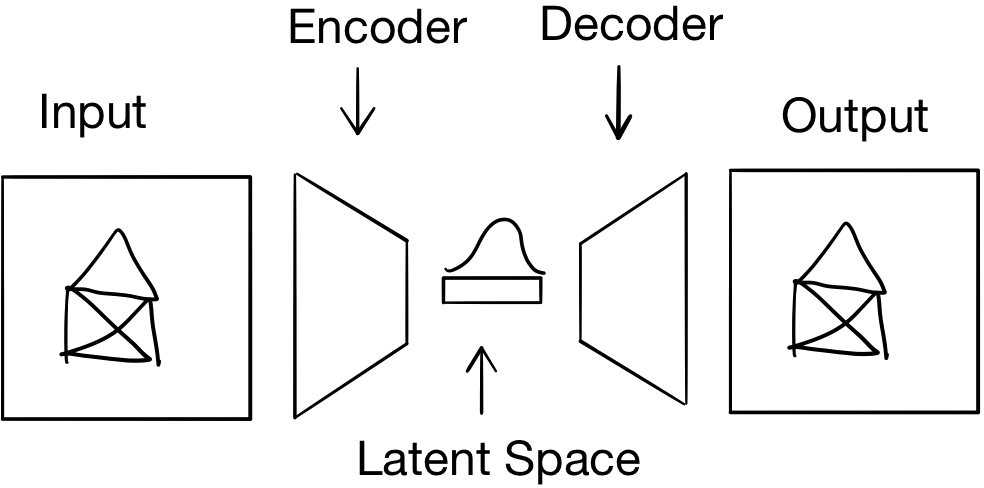
\includegraphics[width=\textwidth]{pres_imgs/vae_sketch.png}
\caption{Abstract Visualization of a VAE}
\label{fig:vae_sketch}
\end{figure}
\end{column}
\end{columns}
\end{frame}
\begin{frame}{The Variational Autoencoder as a Model of the Visual System}
The controllable latent space and the general biological plausibility of CNNs make the VAE an interesting candidate of a model of the visual system.
\end{frame}


\section{Theoretical Background}
\begin{frame}{The Human Visual System}
\begin{columns}
\begin{column}{0.48\textwidth}
The Visual Cortex is mainly hierarchically structured.
The ventral pathway encodes the \textit{what}, the dorsal pathway the \textit{where}~\cite{goodale1992separate}.

\begin{itemize}
\item Simple and complex cells
\item Sparse coding
\end{itemize}
\end{column}
\begin{column}{0.48\textwidth}
\begin{figure}
\centering
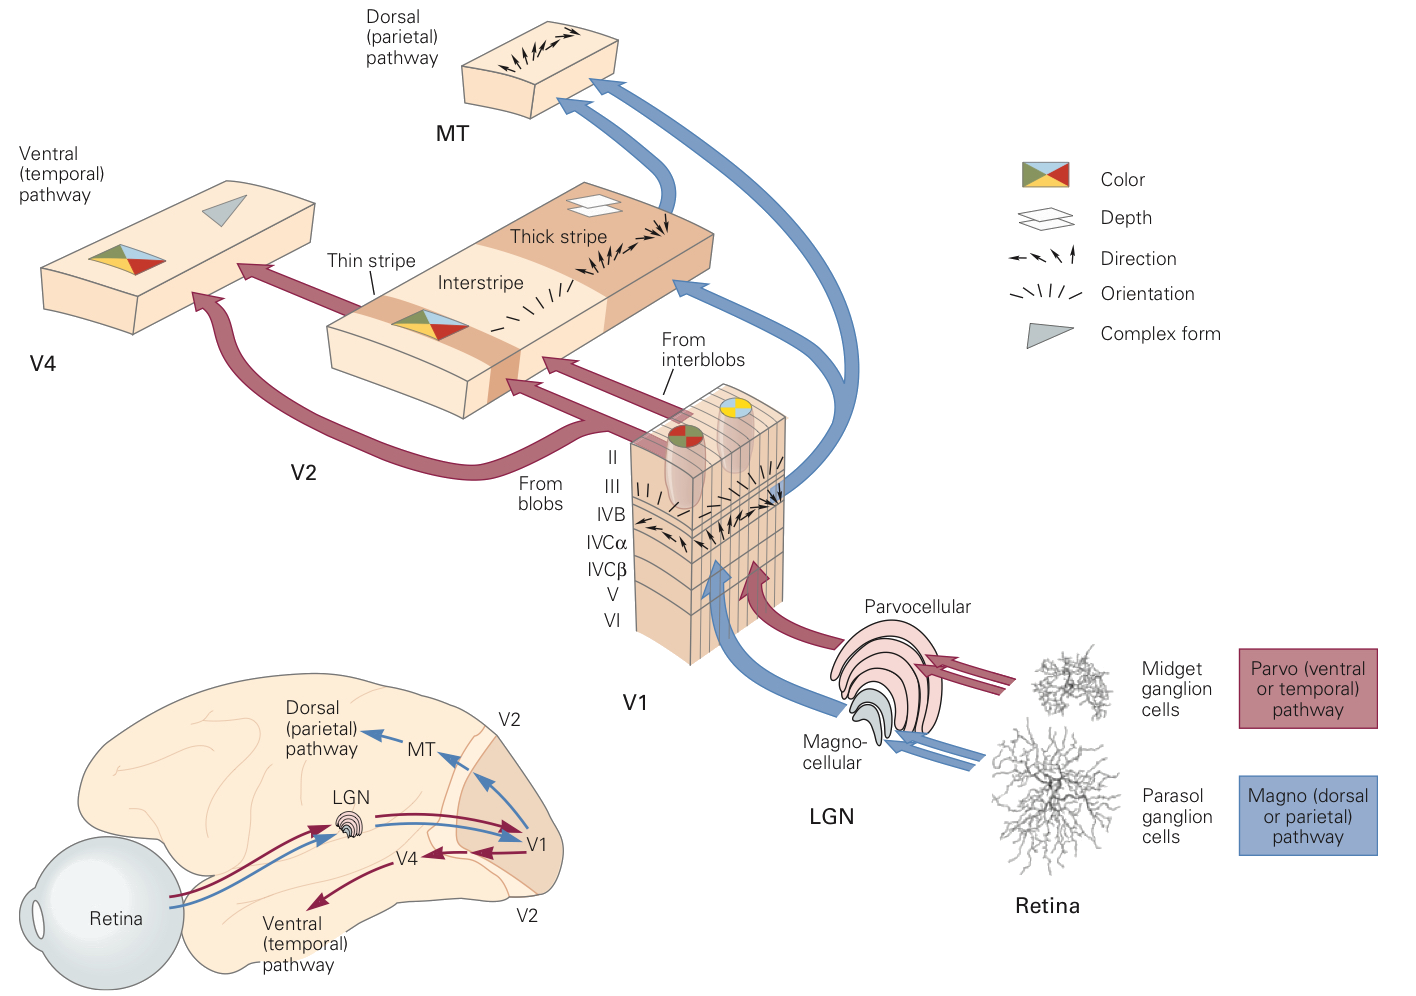
\includegraphics[width=\textwidth]{pres_imgs/ventral_dorsal.png}
\caption{Hierarchical structure of the Visual Cortex, and Ventral and Dorsal Pathways (taken from \cite[p. 571]{mack2013principles})}
\label{fig:figure_ventral_dorsal}
\end{figure}
\end{column}
\end{columns}
\end{frame}
\begin{frame}{Convolutional Neural Networks}
\begin{columns}
\begin{column}{0.48\textwidth}
Convolutions are models of S-cells~\cite{lindsay2020convolutional}.

A subsequent down-scaling introduces translation invariance (C-cells)~\cite{lindsay2020convolutional}.
\end{column}
\begin{column}{0.48\textwidth}
\begin{figure}
\centering
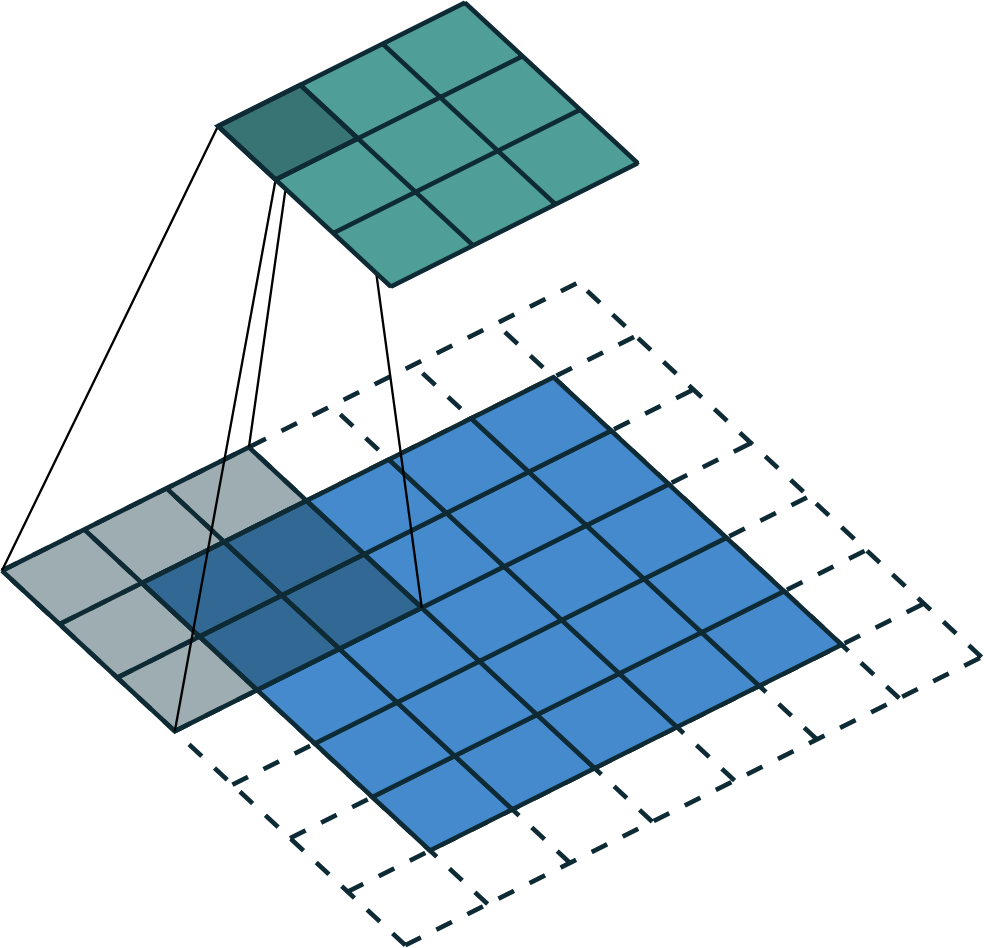
\includegraphics[width=\textwidth]{pres_imgs/convolution_example.png}
\caption{Example of a convolution, taken from \cite{dumoulin2016guide}}
\label{fig:example_convolution}
\end{figure}
\end{column}
\end{columns}
\end{frame}
\begin{frame}{Variational Autoencoders 1}
A VAE has two spaces: $\bm{z}$- and $\bm{x}$-space.
The model learns a joint probability distribution.
\begin{align*}
p(\bm{x}) &= \int p(\bm{x}, \bm{z})d\bm{z}\\
&= \int p(\bm{x}|\bm{z})\,p(\bm{z})d\bm{z}.
\end{align*}
\end{frame}
\begin{frame}{Variational Autoencoders 2}
Given $\bm{x}$, what is the latent space distribution?
\begin{align*}
p(\bm{z}|\bm{x}) &= \frac{p(\bm{x}|\bm{z})p(\bm{z})}{p(\bm{x})} \\
p(\bm{x}) &= \int p(\bm{x}|\bm{z})p(\bm{z})d\bm{z}
\end{align*}
Computing the posterior $p(\bm{z}|\bm{x})$ is intractable!
\end{frame}
\begin{frame}{Variational Autoencoders 3}
\begin{columns}
\begin{column}{0.48\textwidth}
The \textit{true} posterior $p(\bm{z}|\bm{x})$ is approximated by an \textit{inference model} $q_\phi(\bm{z}|\bm{x})$.

VAEs minimize the difference between the true and the approximated posterior.
\end{column}
\begin{column}{0.48\textwidth}
\begin{figure}
\centering
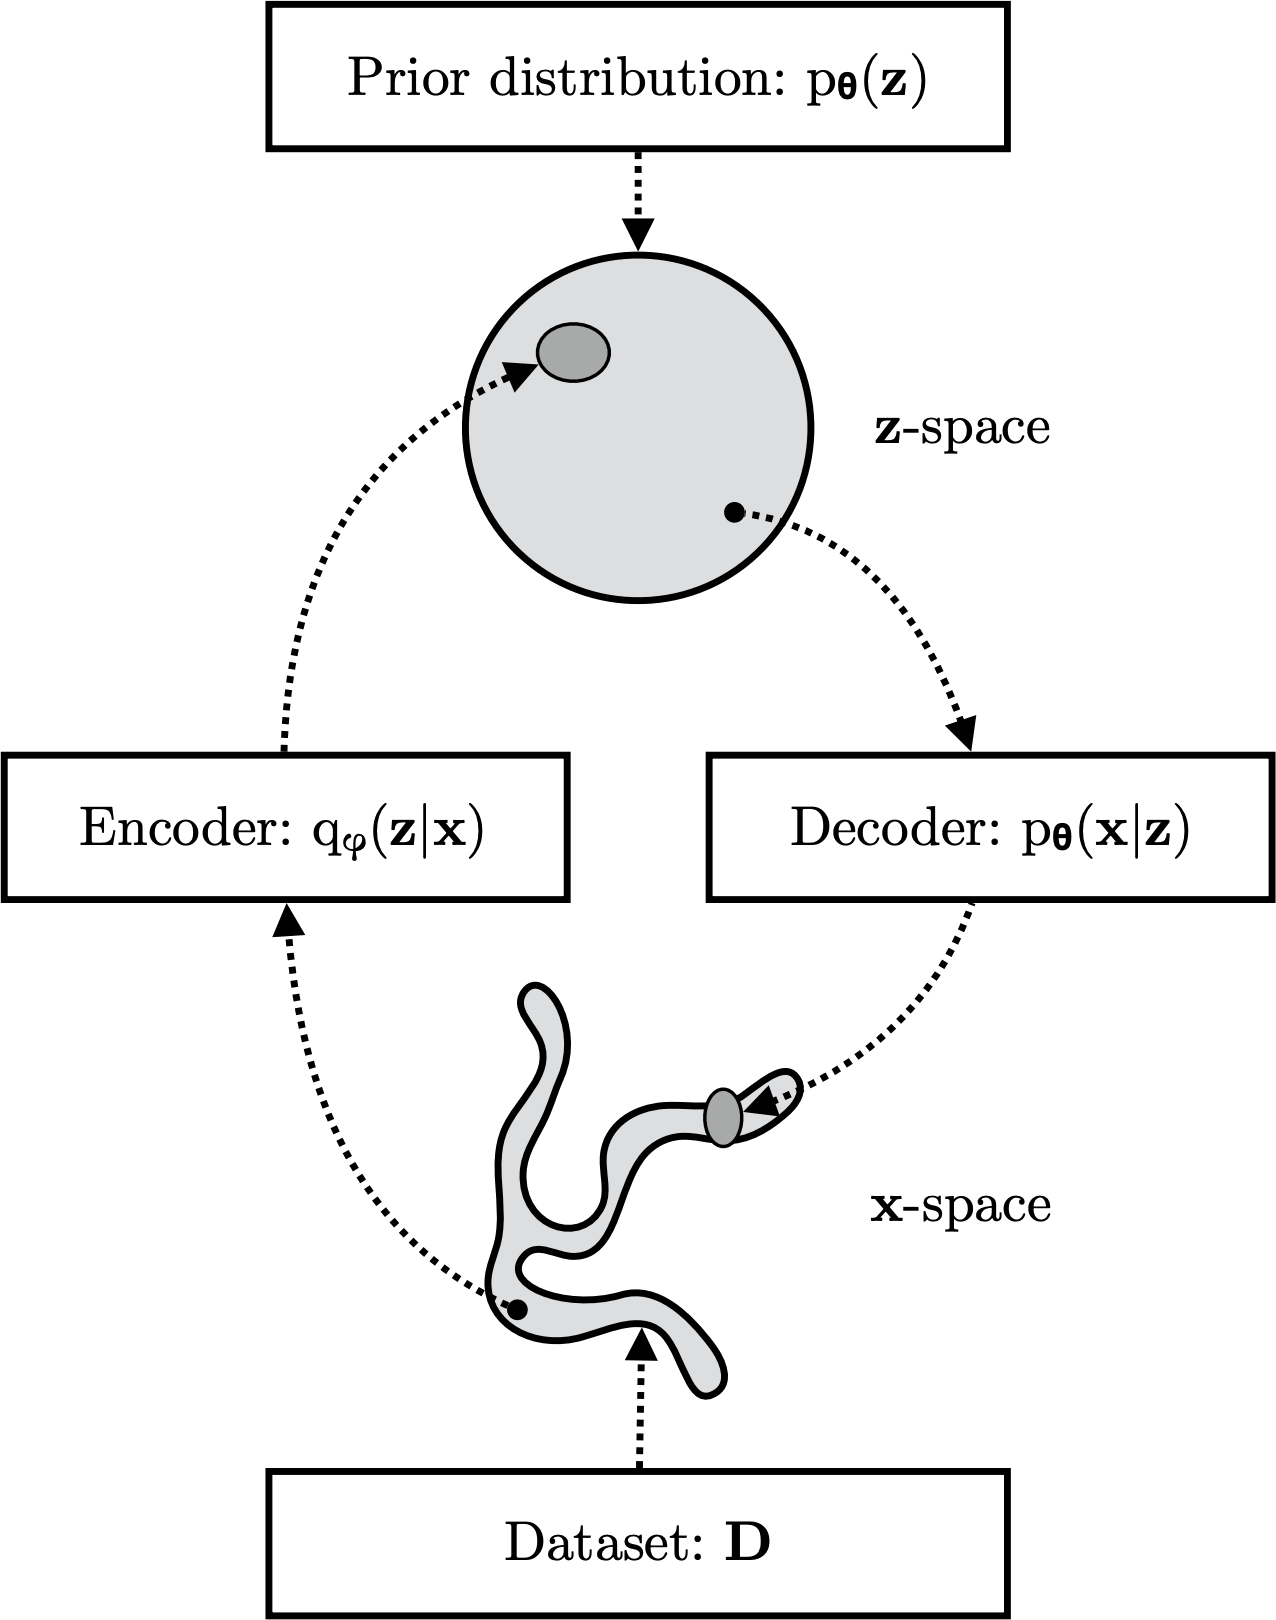
\includegraphics[width=.9\textwidth]{pres_imgs/vae_interplay.png}
\caption{Data and latent distributions in VAEs, taken from~\cite{kingma2019introduction}}
\label{fig:vae_interplay}
\end{figure}
\end{column}
\end{columns}
\end{frame}
\begin{frame}{VAE Training Objective 1}
\begin{align*}
\kldiv{q_\phi(\bm{z}|\bm{x})}{p_\theta(\bm{z}|\bm{x})} &= -\sum_{\bm{z}} q_\phi(\bm{z}|\bm{x}) \log \frac{p_\theta(\bm{z}|\bm{x})}{q_\phi(\bm{z}|\bm{x})} \\
            &= \ldots \\
            &= -\sum_{\bm{z}} q_\phi(\bm{z}|\bm{x}) \log \frac{p_\theta(\bm{x},\bm{z})}{q_\phi(\bm{z}|\bm{x})} + \log p_\theta(\bm{x})
        \end{align*}
        Then
        \begin{align*}
            \underbrace{\vphantom{\sum_{\bm{z}} x}\log p_\theta(\bm{x})}_{\text{constant}} =  \underbrace{\vphantom{\sum_{\bm{z}} x}\kldiv{q_\phi(\bm{z}|\bm{x})}{p_\theta(\bm{z}|\bm{x})}}_{\downarrow}  + \underbrace{\sum_{\bm{z}} q_\phi(\bm{z}|\bm{x}) \log \frac{p_\theta(\bm{x},\bm{z})}{q_\phi(\bm{z}|\bm{x})}}_{\uparrow}.
        \end{align*}
    \end{frame}
    \begin{frame}{VAE Training Objective 2}
        \begin{align*}
            \sum_{\bm{z}} q_\phi(\bm{z}|\bm{x}) \log \frac{p_\theta(\bm{x},\bm{z})}{q_\phi(\bm{z}|\bm{x})} &= \sum_{\bm{z}} q_\phi(\bm{z}|\bm{x}) \log \frac{p_\theta(\bm{x}|\bm{z})p_\theta(\bm{z})}{q_\phi(\bm{z}|\bm{x})}\\
            &= \sum_{\bm{z}} q_\phi(\bm{z}|\bm{x}) \left[ \log p_\theta(\bm{x}|\bm{z}) + \log \frac{p_\theta(\bm{z})}{q_\phi(\bm{z}|\bm{x})} \right]\\
            &= \underbrace{\sum_{\bm{z}} q_\phi(\bm{z}|\bm{x})\log p_\theta(\bm{x}|\bm{z})}_{=\mathbb{E}_{q_\phi(\bm{z}|\bm{x})}\left[ \log p_\theta(\bm{x}|\bm{z}) \right]} + \underbrace{\sum_{\bm{z}} q_\phi(\bm{z}|\bm{x})\log \frac{p_\theta(\bm{z})}{q_\phi(\bm{z}|\bm{x})}}_{=\kldiv{q_\phi(\bm{z}|\bm{x})}{p_\theta(\bm{z})}}. \label{eq:elbo_error_term}
        \end{align*}
    \end{frame}
    \begin{frame}{VAE Training Objective 3}
        \begin{columns}
            \begin{column}{0.48\textwidth}
                $\mathbb{E}_{q_\phi(\bm{z}|\bm{x})}\left[ \log p_\theta(\bm{x}|\bm{z}) \right]$ is basically the mean squared error between input and output.

                The KL-term has a simple closed form if $q_\phi(\bm{z}|\bm{x})$ is independent and $p(\bm{z})$ chosen to be standard normal.
            \end{column}
            \begin{column}{0.48\textwidth}
                \begin{figure}
                    \centering
                    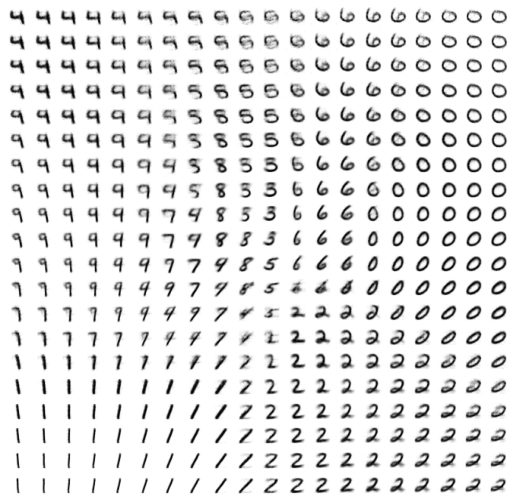
\includegraphics[width=\textwidth]{images/latent_space_traversals/vae_mnist.png}
                    \caption{Latent Space Exploration of a VAE on Hand-Written Digits}
                    \label{fig:vae_mnist}
                \end{figure}
            \end{column}
        \end{columns}
    \end{frame}
    \begin{frame}{Variational Ladder Autoencoder 1}
        \begin{columns}
            \begin{column}{0.48\textwidth}
                Employ multiple latent spaces $\bm{z}_i$ with inference networks of differing capacities.
            \end{column}
            \begin{column}{0.48\textwidth}
                \begin{figure}
                    \centering
                    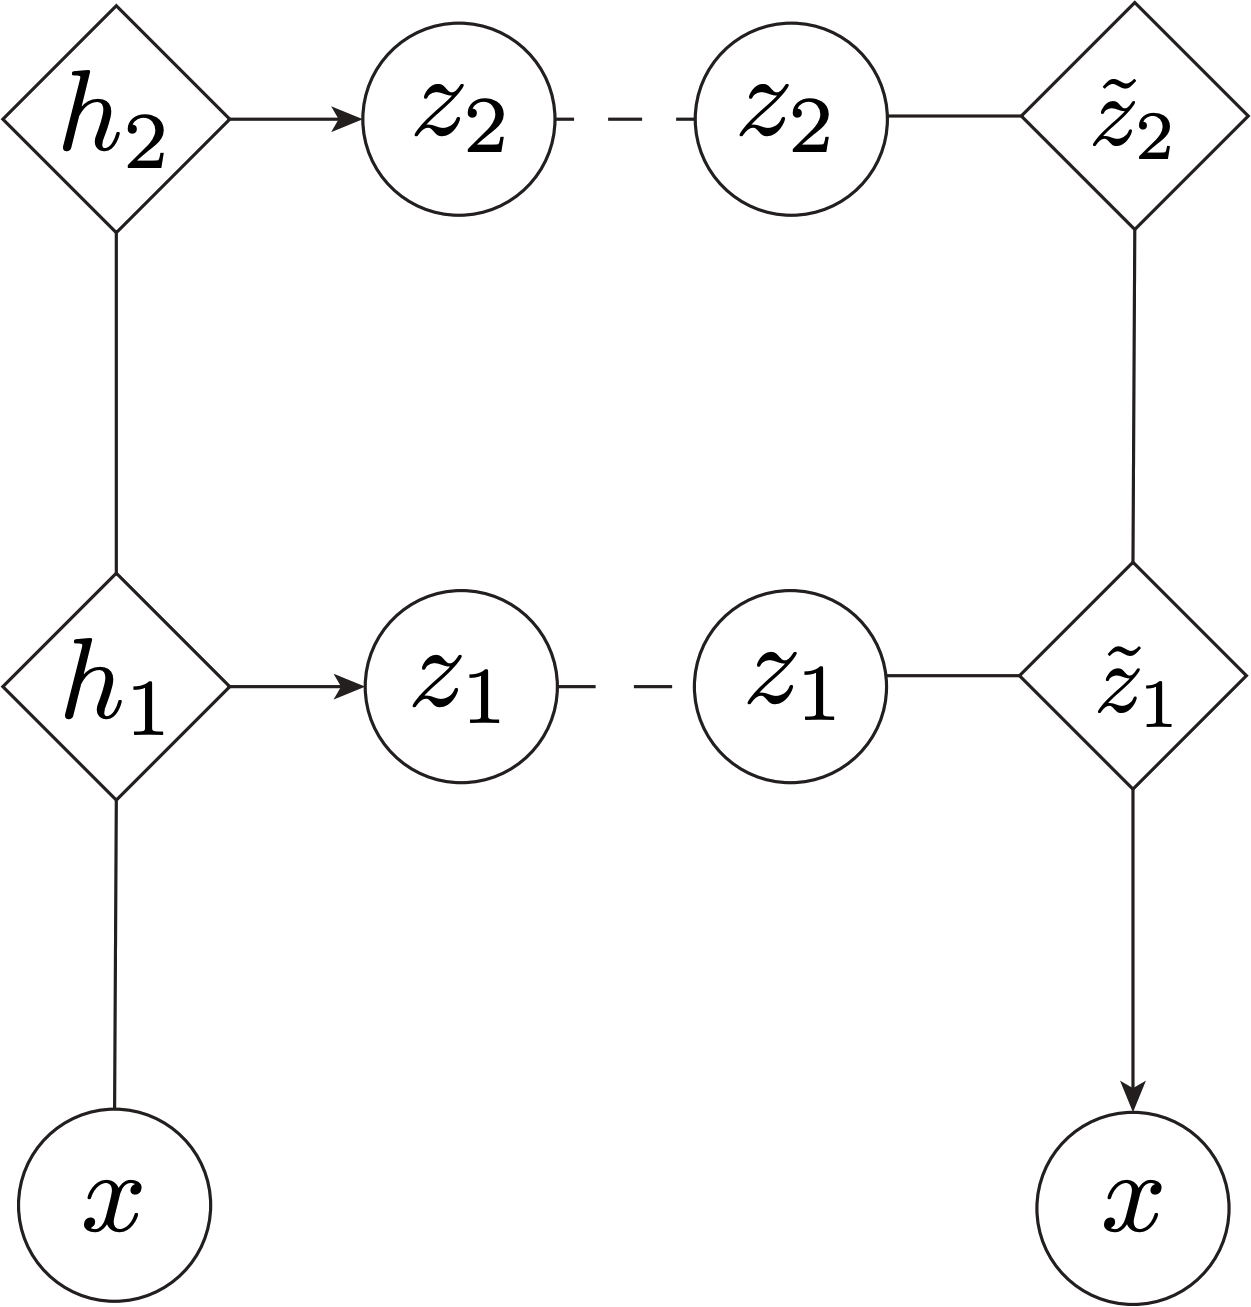
\includegraphics[width=\textwidth]{pres_imgs/vlae_structure.png}
                    \caption{VLAE Structure, taken from~\cite{zhao2017learning}}
                    \label{fig:vae_structure}
                \end{figure}
            \end{column}
        \end{columns}
    \end{frame}
    \begin{frame}{Variational Ladder Autoencoder 2}
        \begin{columns}
            \begin{column}{0.3\textwidth}
                Layers with a less powerful inference network learn lower-level factors of variation.
            \end{column}
            \begin{column}{0.68\textwidth}
                \begin{figure}
                    \centering
                    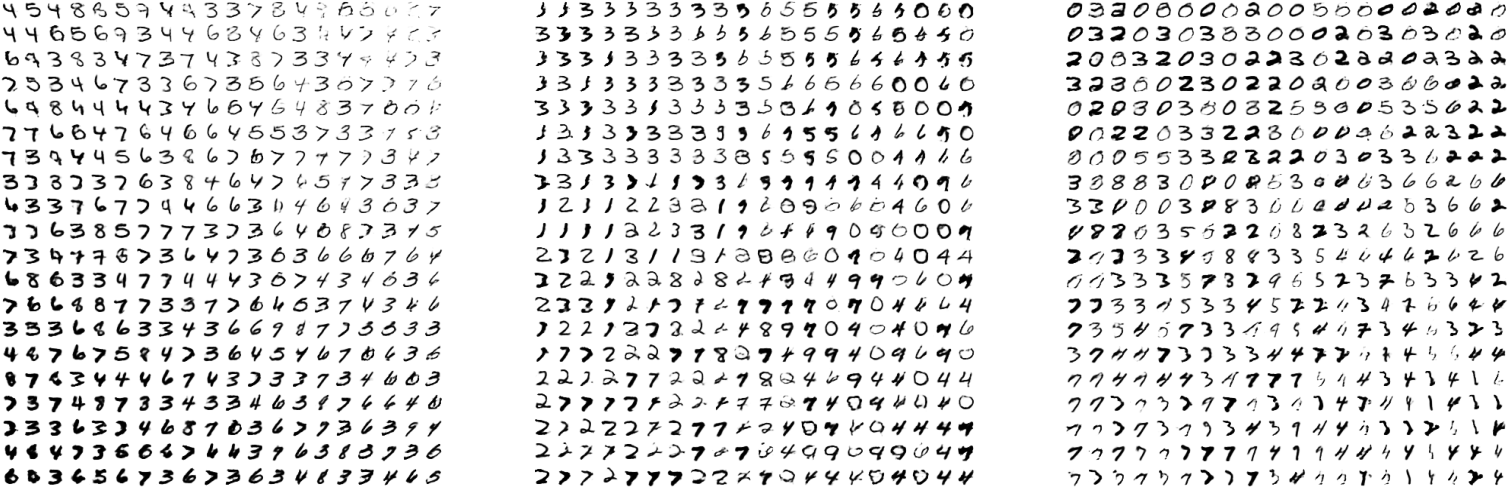
\includegraphics[width=\textwidth]{images/latent_space_traversals/vlae_mnist.png}
                    \caption{Latent Space Exploration of a 3-Layer VLAE on Hand-Written Digits}
                    \label{fig:vlae_mnist}
                \end{figure}
            \end{column}
        \end{columns}
    \end{frame}
    \begin{frame}{Latent Space Disentanglement / Separability}
        \begin{enumerate}
            \item Changing one factor of variation affects only \ldots
            \begin{itemize}
                \item \ldots a single (linear) subspace in the latent space (\textit{Disentanglement}).
                \item \ldots a single layer $\bm{z}_i$ (\textit{Separability}).
            \end{itemize}
            \item Generating $\bm{\tilde{x}}$ by sampling from $\bm{z}$ approximately leads to the data distribution.
        \end{enumerate}
    \end{frame}


    \section{Methods}
    \begin{frame}{Research Questions 1}
        \begin{table}[H]
            \begin{tabularx}{\textwidth}{llX}
                \toprule \\
                \multicolumn{2}{l}{Number} & Question \\
                \midrule \\
                RQ1 &    & Are VAEs or VLAEs related to the visual cortex in terms of \ldots                                      \\
                & a) & \hspace{1cm} \ldots the emergence of Gabor wavelets?                                                   \\
                & b) & \hspace{1cm} \ldots sparse coding?                                                                     \\
                RQ2 &    & Do VAEs or VLAEs fulfil the requirements of latent space disentanglement or latent space separability? \\
                RQ3 &    & Can VAEs or VLAEs represent both continuous and categorical factors of variation in the latent space?  \\
                RQ4 &    & How do VAEs and VLAEs represent lower factors of variation in the latent space?                        \\
            \end{tabularx}
        \end{table}
    \end{frame}
    \begin{frame}{Research Questions 2}
        \begin{table}[H]
\begin{tabularx}{\textwidth}{llX}
RQ5 & & Do VAEs or VLAEs learn independent factors of variation independently in the latent space?              \\
RQ6 & & Are the latent spaces of VLAEs independent in terms of generated images?                                \\
RQ7 & & Do VAE/VLAE-generated images resemble the data distribution?                                            \\
RQ8 & & Is the discriminative loss superior to the pixel-wise loss in terms of the previous research questions? \\
\bottomrule
\end{tabularx}
\caption{Research Questions}
\end{table}
\end{frame}
\begin{frame}{Models}
\fontsize{6pt}{7.2}\selectfont
\begin{table}[H]
\centering
\begin{tabularx}{\textwidth}{lXXXXX}
\toprule
model name              & dataset        & \parbox[t]{1cm}{\fontsize{6pt}{7.2}\raggedleft input/output\\size}       & \parbox[t]{1cm}{\fontsize{6pt}{7.2}\raggedleft latent\\space\\size} & \parbox[t]{1cm}{\fontsize{6pt}{7.2}\raggedleft reconstruction\\term weight} & \parbox[t]{1cm}{\fontsize{6pt}{7.2}\raggedleft feature\\map\\reduction factor} \\
\midrule
\textsc{Mnist}-VAE & \textsc{Mnist} & $28\times 28\times 1$   & 2                 & 10,000                     & 1                            \\
(dSprites/10,000)-VAE       & dSprites       & $64\times 64\times 1$   & 10                & 10,000                     & 1                            \\
7,500-VAE          & dSprites       & $64\times 64\times 1$   & 10                & 7,500                      & 1                            \\
6,250-VAE          & dSprites       & $64\times 64\times 1$   & 10                & 6,250                      & 1                            \\
5,000-VAE          & dSprites       & $64\times 64\times 1$   & 10                & 5,000                      & 1                            \\
3,750-VAE          & dSprites       & $64\times 64\times 1$   & 10                & 3,750                      & 1                            \\
dSprites-VAE-dim6  & dSprites       & $64\times 64\times 1$   & 6                 & 10,000                     & 1                            \\
CelebA-VAE         & CelebA         & $128\times 128\times 3$ & 8                 & 3,750                      & 1                            \\
\midrule
\textsc{Mnist}-VLAE(-factor-1) & \textsc{Mnist} & $28\times 28\times 1$ & 2,2,2 & 10,000 & 1 \\
\textsc{Mnist}-VLAE-factor-2 & \textsc{Mnist} & $28\times 28\times 1$ & 2,2,2 & 10,000 & 2 \\
\textsc{Mnist}-VLAE-factor-3 & \textsc{Mnist} & $28\times 28\times 1$ & 2,2,2 & 10,000 & 3 \\
dSprites-VLAE & dSprites & $64\times 64\times 1$ & 4,4,4 & 10,000 & 1 \\
dSprites-VLAE-dim2 & dSprites & $64\times 64\times 1$ & 2,2,2 & 10,000 & 1 \\
CelebA-VLAE & CelebA & $128\times 128\times 3$ & 2,2,2 & 10,000 & 1 \\
\midrule
\textsc{Mnist}-VAE-GAN & \textsc{Mnist} & $28\times 28\times 1$ & 2 & 10,000 & 1\\
dSprites-VAE-GAN & dSprites & $64\times 64\times 1$ & 10 & 10,000 & 1\\
CelebA-VAE-GAN & CelebA & $128\times 128\times 3$ & 8 & 10,000 & 1\\
\end{tabularx}
\end{table}
\end{frame}
\begin{frame}
\fontsize{6pt}{7.2}\selectfont
\begin{table}[H]
\centering
\begin{tabularx}{\textwidth}{lXXXXX}
\textsc{Mnist}-VLAE-GAN & \textsc{Mnist} & $28\times 28\times 1$ & 2,2,2 & 10,000 & 1\\
dSprites-VLAE-GAN & dSprites & $64\times 64\times 1$ & 4,4,4 & 10,000 & 1\\
CelebA-VLAE-GAN & CelebA & $128\times 128\times 3$ & 2,2,2 & 10,000 & 1\\
\midrule
AlexNet Classifier & ImageNet & $224\times 224\times 3$ & -- & -- & 1\\
\midrule
AlexNet VAE & ImageNet & $224\times 224\times 3$ & 2000 & 10,000 & 1\\
\bottomrule
\end{tabularx}
\caption[Models Overview]{Overview of all models with important parameters.}
\end{table}
\end{frame}
\begin{frame}{Datasets}
\begin{itemize}
\item CelebA
\item ImageNet
\item \textsc{Mnist}
\item Morpho-\textsc{Mnist}
\item dSprites
\end{itemize}
\end{frame}
\section{Results}
\subsection{Gabor Wavelets in First Layer}
\begin{frame}{Gabor Wavelets in First Layer}
\begin{columns}
\begin{column}{0.48\textwidth}
\begin{figure}
\centering
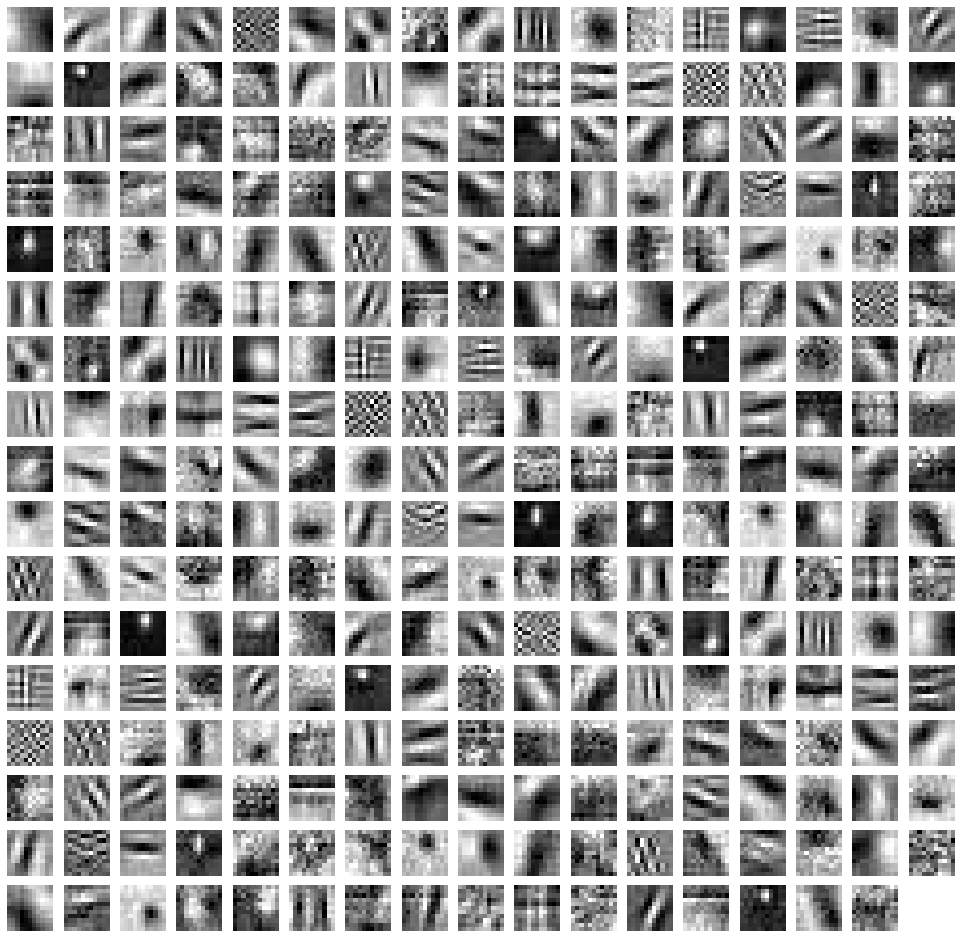
\includegraphics[width=\textwidth]{images/alexnet_classification_l1_kernels.png}
\caption{Layer 1 Kernels in Classification Network}
\end{figure}
\end{column}
\begin{column}{0.48\textwidth}
\begin{figure}
\centering
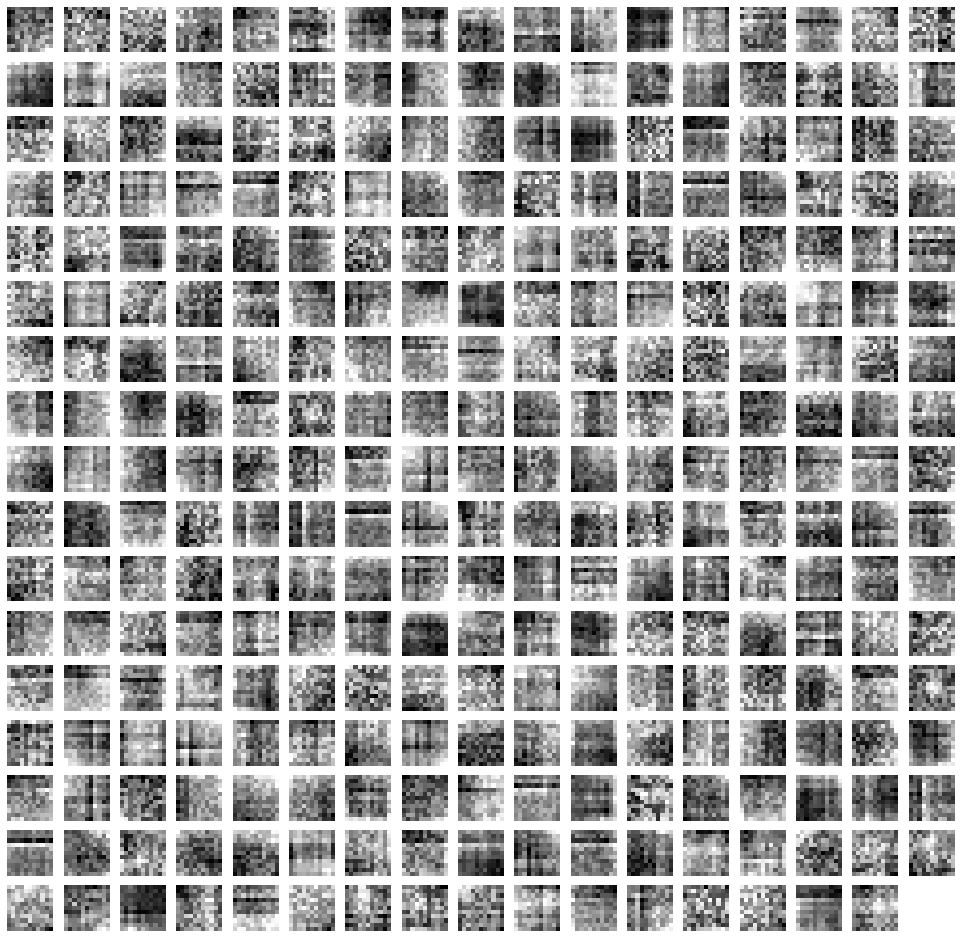
\includegraphics[width=\textwidth]{images/alexnet_vae_l1_kernels.png}
\caption{Layer 1 Kernels in AlexNet-VAE}
\end{figure}
\end{column}
\end{columns}
\end{frame}
\subsection{Latent Space Entanglement and Categorical Factors of Variation}
\begin{frame}
\begin{figure}
\centering
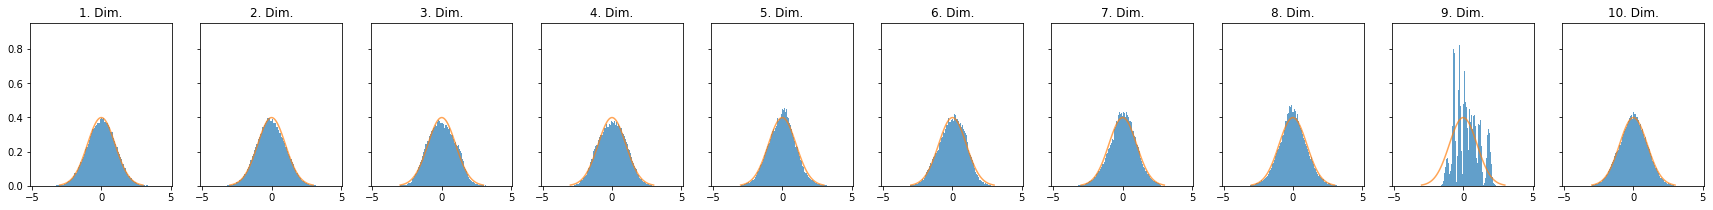
\includegraphics[width=\textwidth]{images/latent_space_entanglement/vae_dsprites_lf_10000_dist.png}
\caption[VAE Latent Space Distribution - dSprites]{dSprites-VAE - posterior distribution}
\end{figure}
\end{frame}
\begin{frame}
\begin{figure}
\centering
\begin{subfigure}{\textwidth}
\centering
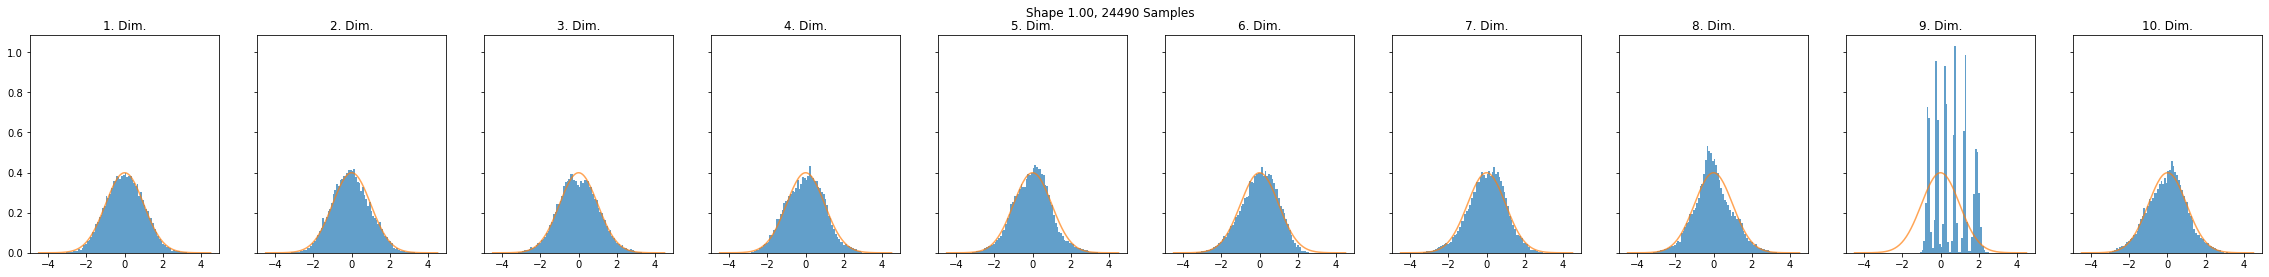
\includegraphics[width=\textwidth]{images/latent_space_entanglement/vae_dsprites_lf_10000_dist_shape_1.png}
\caption{Latent space distribution of images with shape \textit{Square}}
\end{subfigure}
\begin{subfigure}{\textwidth}
\centering
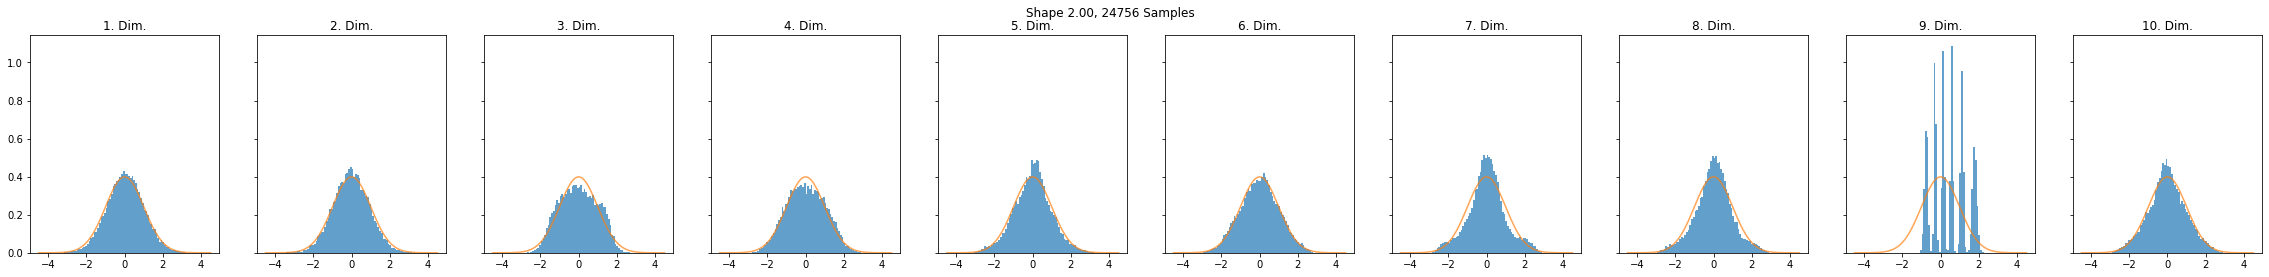
\includegraphics[width=\textwidth]{images/latent_space_entanglement/vae_dsprites_lf_10000_dist_shape_2.png}
\caption{Latent space distribution of images with shape \textit{Ellipse}}
\end{subfigure}
\begin{subfigure}{\textwidth}
\centering
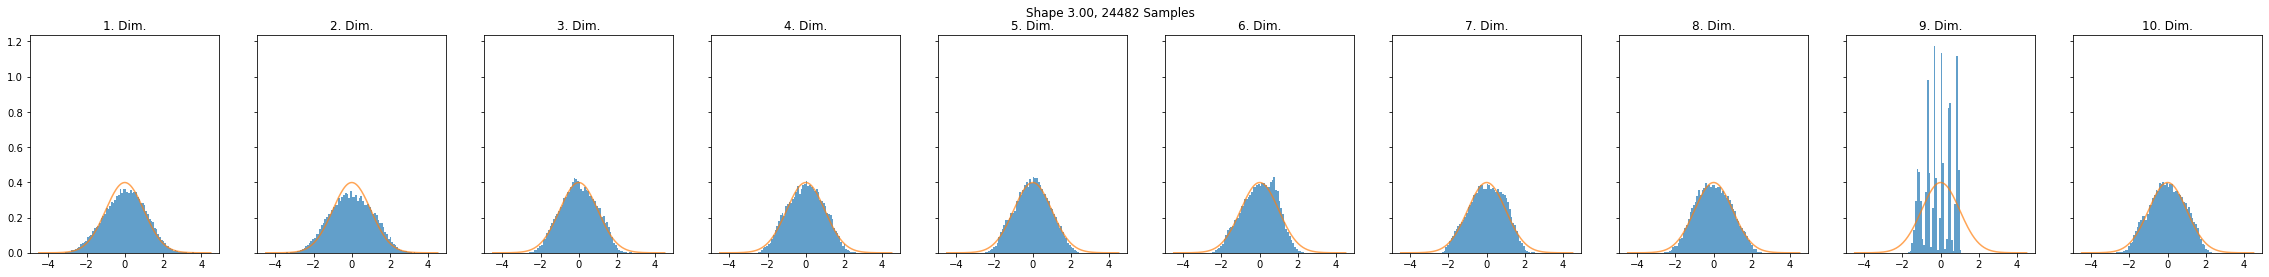
\includegraphics[width=\textwidth]{images/latent_space_entanglement/vae_dsprites_lf_10000_dist_shape_3.png}
\caption{Latent space distribution of images with shape \textit{Heart}}
\end{subfigure}
\caption[VAE Latent Space Distribution - dSprites Shapes]{Histogram of dSprites images with a certain shape from the validation set in 100 bins}
\end{figure}
\end{frame}
\begin{frame}
\begin{figure}
\centering
\begin{subfigure}{\textwidth}
\centering
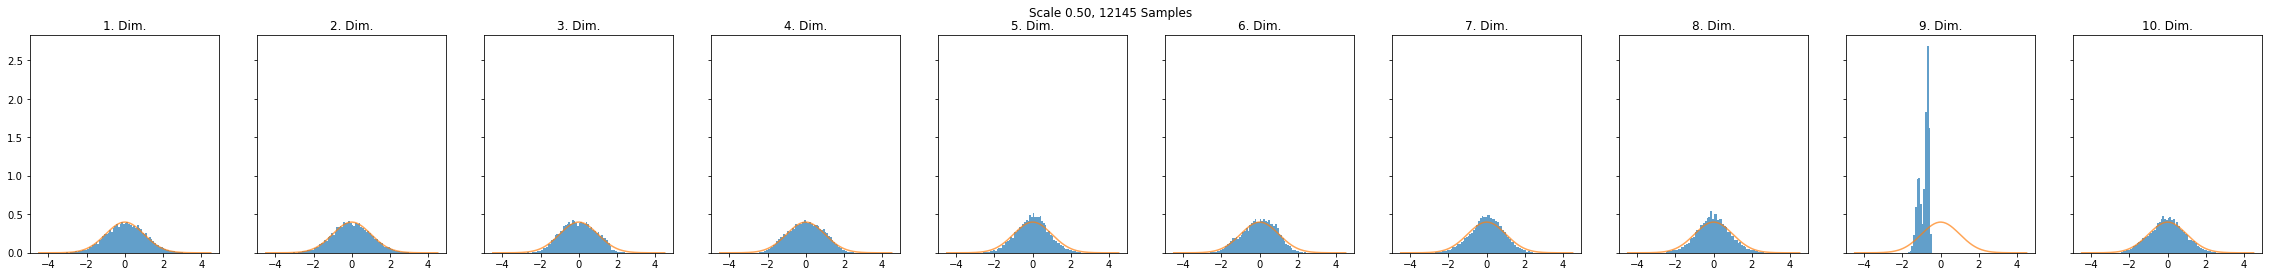
\includegraphics[width=\textwidth]{images/latent_space_entanglement/vae_dsprites_lf_10000_dist_scale_0_5.png}
\caption{Latent space distribution of images with scale = 0.5}
\end{subfigure}
\begin{subfigure}{\textwidth}
\centering
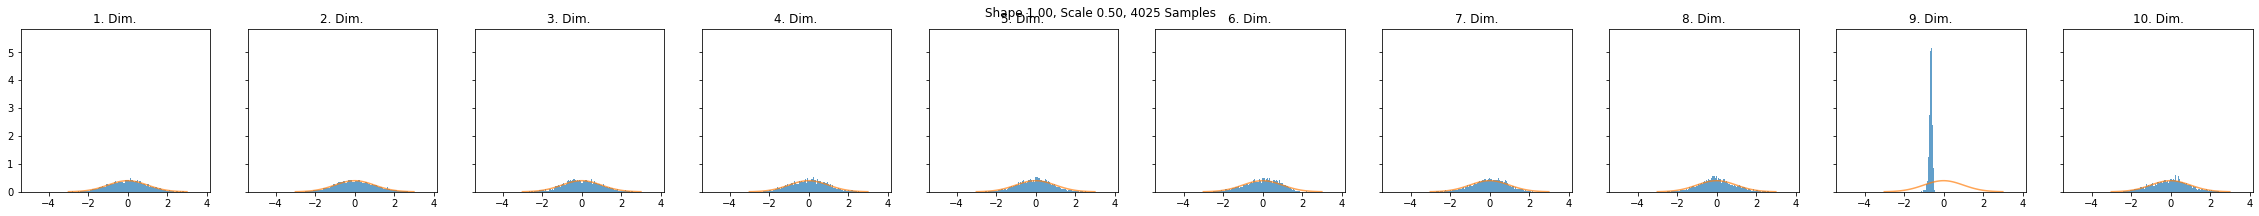
\includegraphics[width=\textwidth]{images/latent_space_entanglement/vae_dsprites_lf_10000_dist_shape_1_scale_0_5.png}
\caption{Latent space distribution of images with scale = 0.5 and shape \textit{Square}}
\end{subfigure}
\begin{subfigure}{\textwidth}
\centering
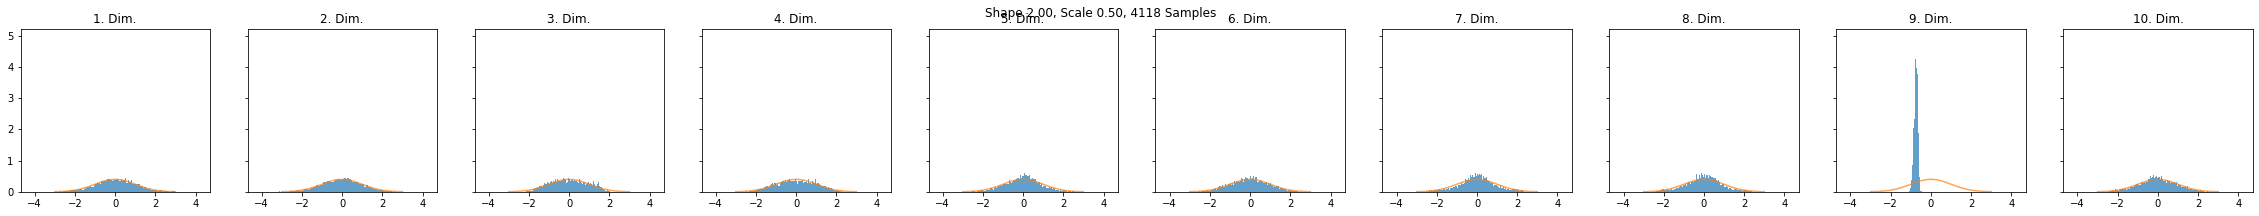
\includegraphics[width=\textwidth]{images/latent_space_entanglement/vae_dsprites_lf_10000_dist_shape_2_scale_0_5.png}
\caption{Latent space distribution of images with scale = 0.5 and shape \textit{Ellipse}}
\end{subfigure}
\begin{subfigure}{\textwidth}
\centering
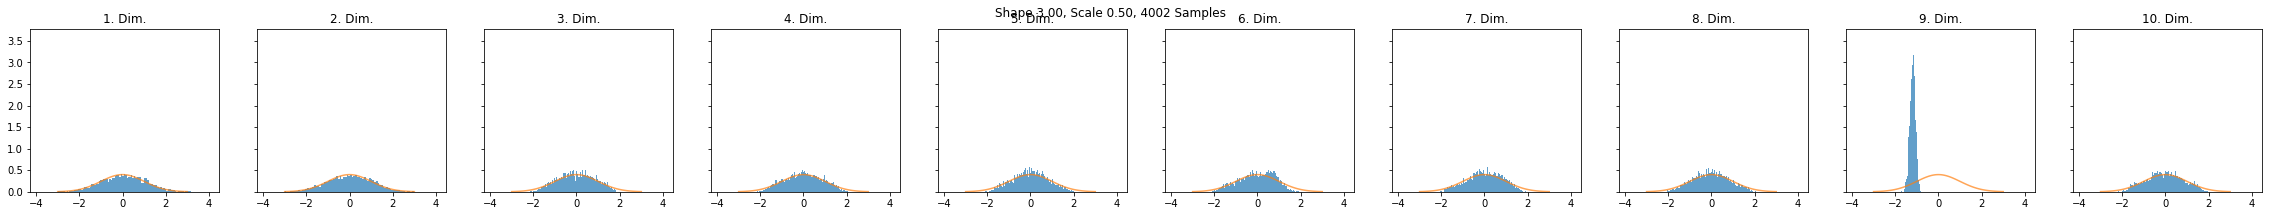
\includegraphics[width=\textwidth]{images/latent_space_entanglement/vae_dsprites_lf_10000_dist_shape_3_scale_0_5.png}
\caption{Latent space distribution of images with scale = 0.5 and shape \textit{Heart}}
\end{subfigure}
\caption[VAE Latent Space Distribution - dSprites Scale and Shapes]{Posterior distribution for dSprites images with scale = 0.5 and different shapes from the validation set in 100 bins}
\end{figure}
\end{frame}
\begin{frame}{PPL - Different Reconstruction Term Weights}
\begin{table}
\centering
\begin{tabular}{lrr}
\toprule
Model           & mean PPL & standard deviation \\
\midrule
10,000-VAE & 936.257       & 779.098            \\
7,500-VAE  & 2834.674      & 567.933            \\
6,250-VAE  & 4498.156      & 1091.255           \\
5,000-VAE  & 173.533       & 35.896             \\
3,750-VAE  & 258.326       & 49.117             \\
\bottomrule
\end{tabular}
\caption[dSprites-VAEs: Perceptual Path Lengths]{Perceptual path lengths for the different models latent spaces}
\end{table}
\end{frame}
\subsection{Latent Space Embeddings}
\begin{frame}
\begin{figure}
\centering
\begin{subfigure}{.32\textwidth}
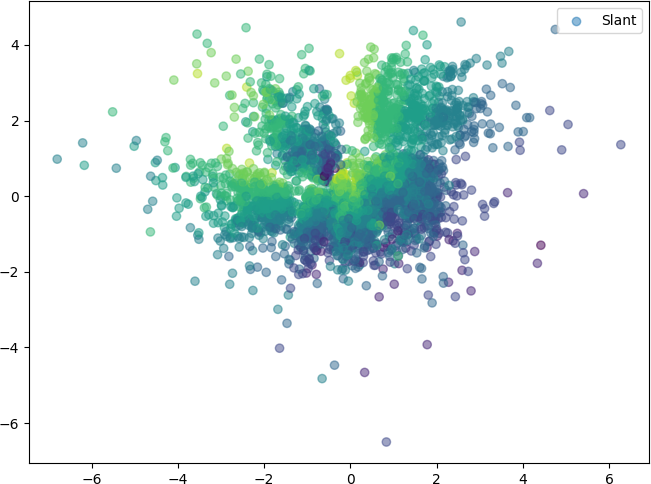
\includegraphics[width=\textwidth]{images/latent_spaces/mnist/vae/embeddings_mu_0.png}
\caption{Slant}
\end{subfigure}
\hfill
\begin{subfigure}{.32\textwidth}
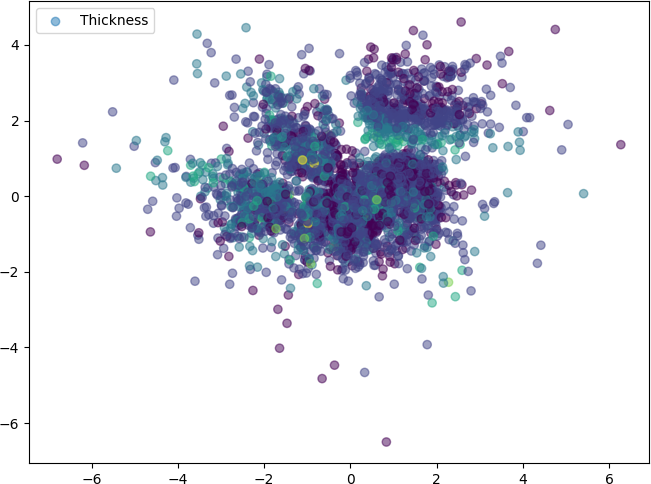
\includegraphics[width=\textwidth]{images/latent_spaces/mnist/vae/embeddings_mu_1.png}
\caption{Thickness}
\end{subfigure}
\hfill
\begin{subfigure}{.32\textwidth}
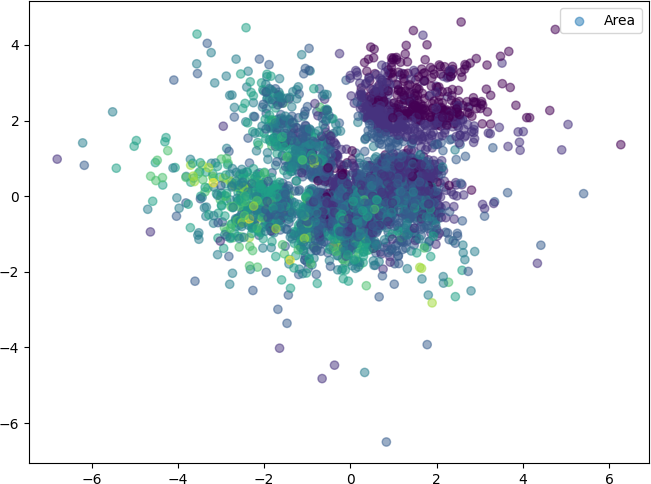
\includegraphics[width=\textwidth]{images/latent_spaces/mnist/vae/embeddings_mu_2.png}
\caption{Area}
\end{subfigure}
\hfill
\begin{subfigure}{.24\textwidth}
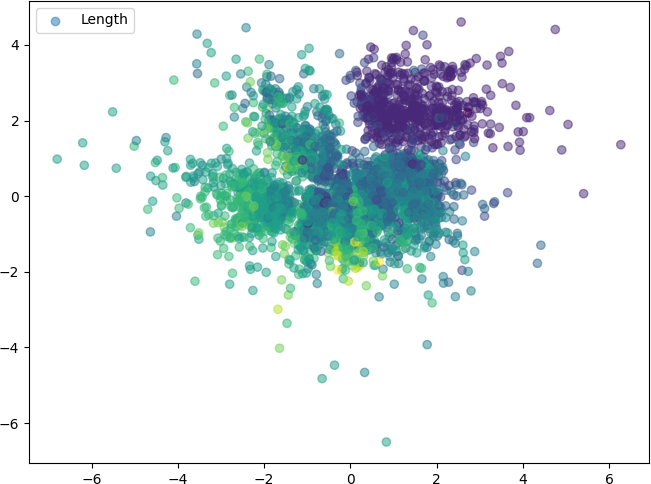
\includegraphics[width=\textwidth]{images/latent_spaces/mnist/vae/embeddings_mu_3.png}
\caption{Length}
\end{subfigure}
\hfill
\begin{subfigure}{.24\textwidth}
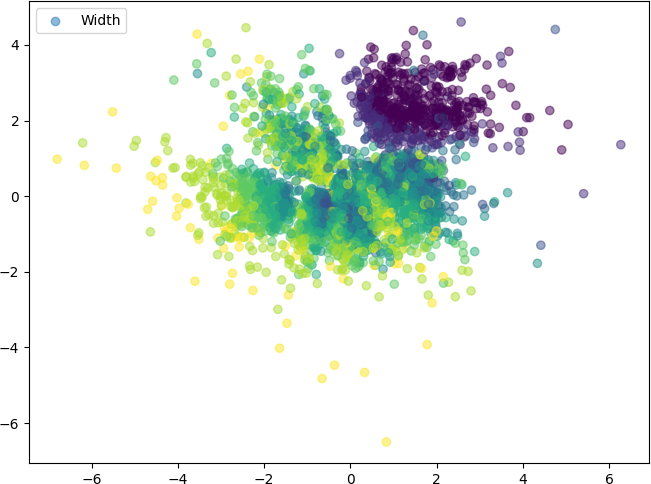
\includegraphics[width=\textwidth]{images/latent_spaces/mnist/vae/embeddings_mu_4.png}
\caption{Width}
\end{subfigure}
\hfill
\begin{subfigure}{.24\textwidth}
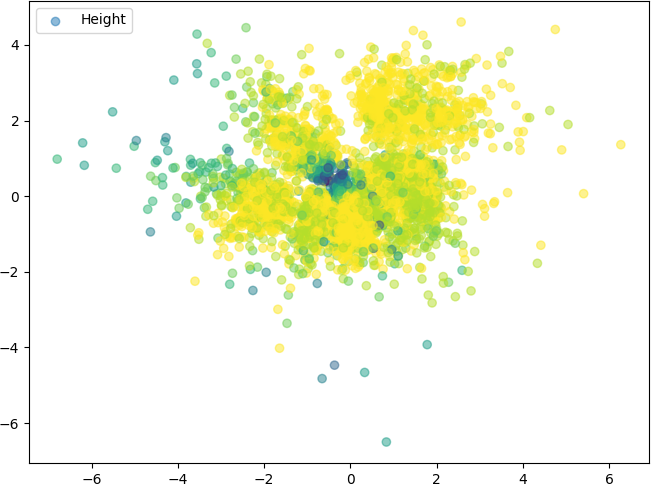
\includegraphics[width=\textwidth]{images/latent_spaces/mnist/vae/embeddings_mu_5.png}
\caption{Height}
\end{subfigure}
\hfill
\begin{subfigure}{.24\textwidth}
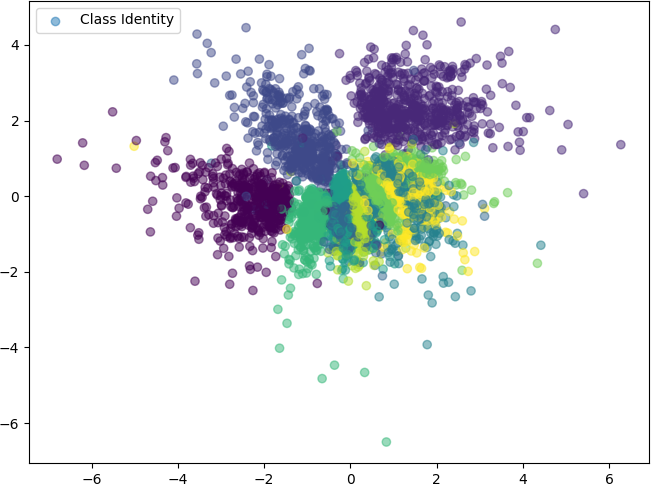
\includegraphics[width=\textwidth]{images/latent_spaces/mnist/vae/embeddings_mu_6.png}
\caption{Identity}
\end{subfigure}
\caption{Colored Latent Space - \textsc{Mnist}-VAE}
\end{figure}
\end{frame}
\begin{frame}
\begin{figure}
\centering
\foreach \i in {1,2,3}{
\begin{adjustbox}{valign=T}
\begin{subfigure}{.24\textwidth}
\includegraphics[width=\textwidth]{images/latent_spaces/mnist/vlae/embeddings_mu_\i_0.png}
\end{subfigure}
\end{adjustbox}
\hfill
\begin{adjustbox}{valign=T}
\begin{subfigure}{.24\textwidth}
\includegraphics[width=\textwidth]{images/latent_spaces/mnist/vlae/embeddings_mu_\i_1.png}
\end{subfigure}
\end{adjustbox}
\hfill
\begin{adjustbox}{valign=T}
\begin{subfigure}{.24\textwidth}
\includegraphics[width=\textwidth]{images/latent_spaces/mnist/vlae/embeddings_mu_\i_2.png}
\end{subfigure}
\end{adjustbox}
\hfill
\begin{adjustbox}{valign=T}
\begin{subfigure}{.24\textwidth}
\includegraphics[width=\textwidth]{images/latent_spaces/mnist/vlae/embeddings_mu_\i_6.png}
\end{subfigure}
\end{adjustbox}}
\caption[\textsc{Mnist}-VLAE Latent Space]{Latent space colored by Slant, Thickness, Area, Identity of \textsc{Mnist}-VLAE}
\end{figure}
\end{frame}
\begin{frame}
\begin{figure}
\centering
\begin{adjustbox}{valign=T}
\begin{subfigure}{.19\textwidth}
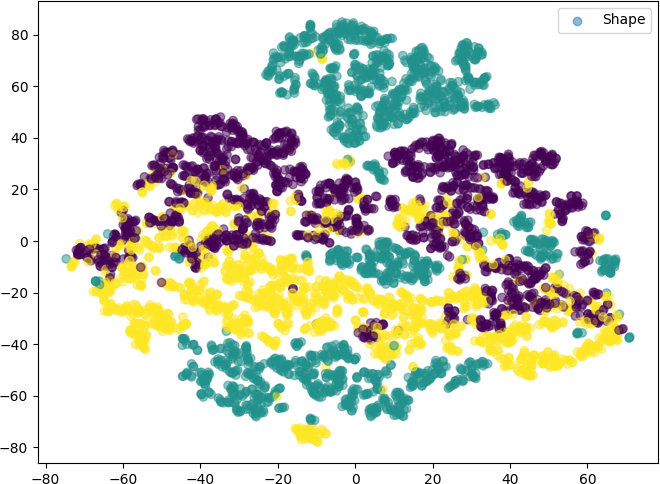
\includegraphics[width=\textwidth]{images/latent_spaces/dsprites/vae/embeddings_mu_0.png}
\caption{Latent space colored by object shape}
\end{subfigure}
\end{adjustbox}
\hfill
\begin{adjustbox}{valign=T}
\begin{subfigure}{.19\textwidth}
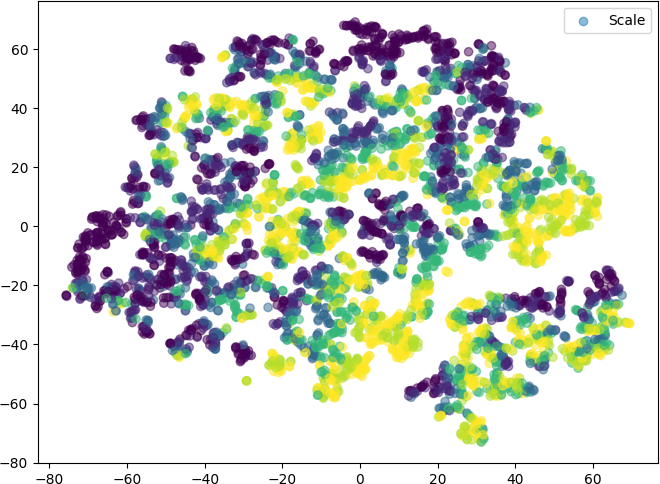
\includegraphics[width=\textwidth]{images/latent_spaces/dsprites/vae/embeddings_mu_1.png}
\caption{Latent space colored by object scale}
\label{subfig:vae_embedding_dsprites_scale}
\end{subfigure}
\end{adjustbox}
\hfill
\begin{adjustbox}{valign=T}
\begin{subfigure}{.19\textwidth}
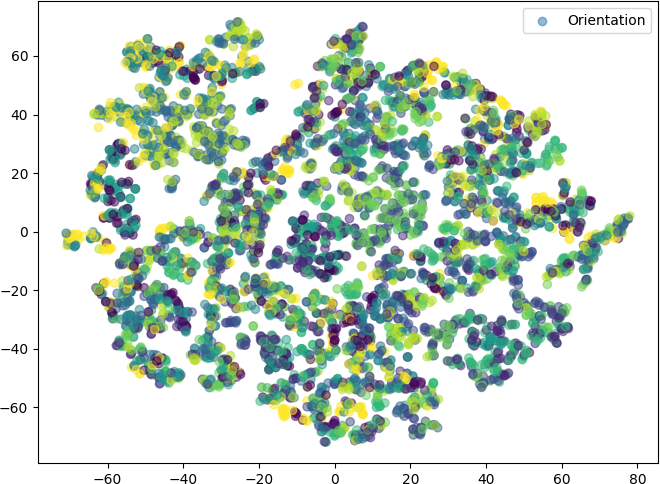
\includegraphics[width=\textwidth]{images/latent_spaces/dsprites/vae/embeddings_mu_2.png}
\caption{Latent space colored by object orientation}
\label{subfig:vae_embedding_dsprites_orientation}
\end{subfigure}
\end{adjustbox}
\hfill
\begin{adjustbox}{valign=T}
\begin{subfigure}{.19\textwidth}
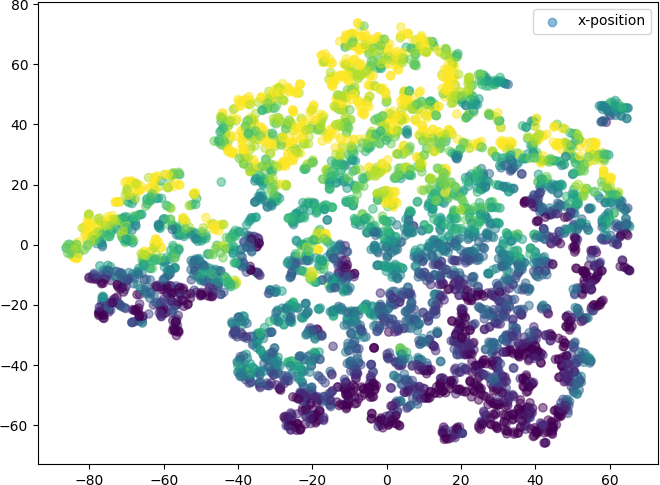
\includegraphics[width=\textwidth]{images/latent_spaces/dsprites/vae/embeddings_mu_3.png}
\caption{Latent space colored by object $x$-position}
\end{subfigure}
\end{adjustbox}
\hfill
\begin{adjustbox}{valign=T}
\begin{subfigure}{.19\textwidth}
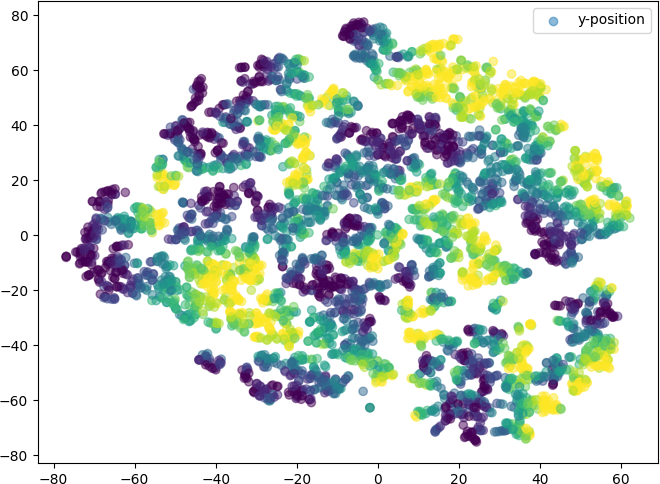
\includegraphics[width=\textwidth]{images/latent_spaces/dsprites/vae/embeddings_mu_4.png}
\caption{Latent space colored by object $y$-position}
\end{subfigure}
\end{adjustbox}
\caption{t-SNE-reduced latent space embeddings colored by different means of dSprites-VAE-dim6}
\end{figure}
\end{frame}
\subsection{Latent Space Explorations}
\begin{frame}
\begin{figure}
\centering
\begin{subfigure}{.45\textwidth}
\centering
% include first image
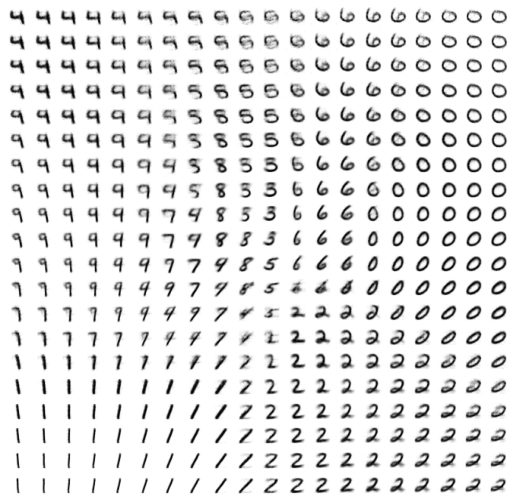
\includegraphics[width=\textwidth]{images/latent_space_traversals/vae_mnist.png}
\caption{VAE latent space exploration from $z_i=-3$ to $z_i=3$ in both $z$ dimensions}
\end{subfigure}
\hfill
\begin{subfigure}{.45\textwidth}
\centering
% include second image
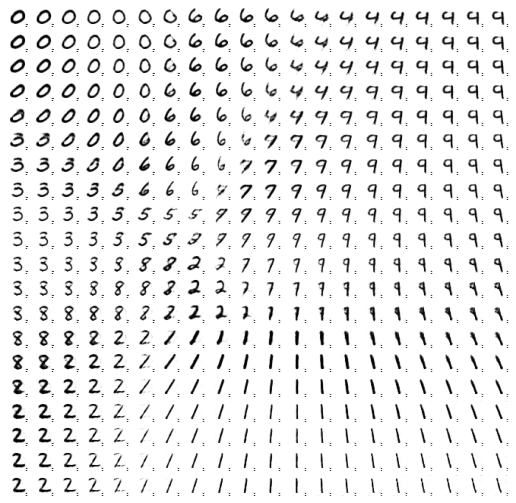
\includegraphics[width=\textwidth]{images/latent_space_traversals/vae_gan_mnist.png}
\caption{VAE-GAN latent space exploration from $z_i=-3$ to $z_i=3$ in both $z$ dimensions}
\end{subfigure}
\caption{Latent space exploration for VAE models on \textsc{Mnist}}
\end{figure}
\end{frame}
\begin{frame}
\begin{figure}
\centering
\begin{subfigure}{\textwidth}
\centering
% include second image
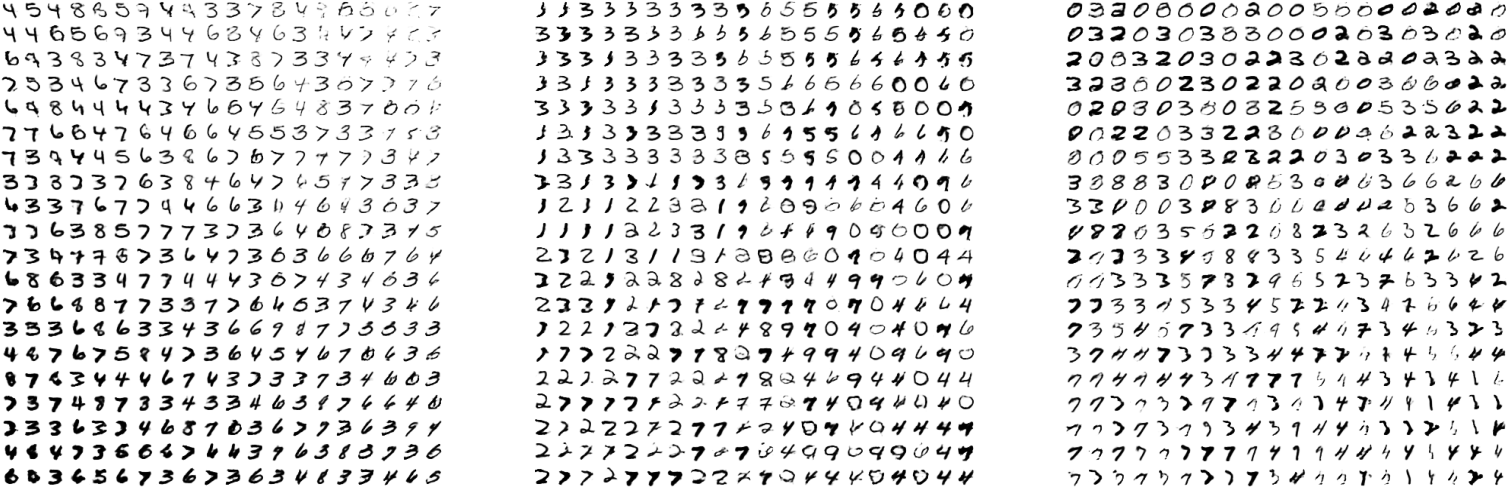
\includegraphics[width=\textwidth]{images/latent_space_traversals/vlae_mnist.png}
\end{subfigure}
\begin{subfigure}{\textwidth}
\centering
% include second image
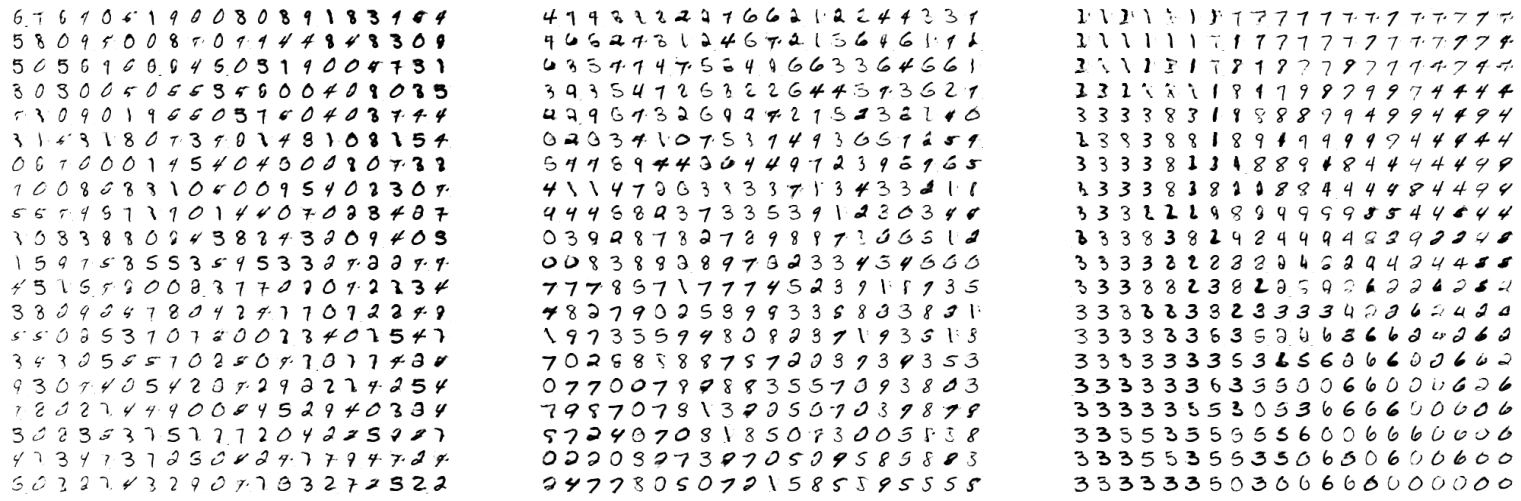
\includegraphics[width=\textwidth]{images/latent_space_traversals/vlae_gan_mnist.png}
\end{subfigure}
\caption{Latent space exploration for VLAE (top) and VLAE-GAN (bottom) on \textsc{Mnist}}
\end{figure}
\end{frame}
\begin{frame}
\begin{figure}
\centering
\begin{subfigure}{.48\textwidth}
% include second image
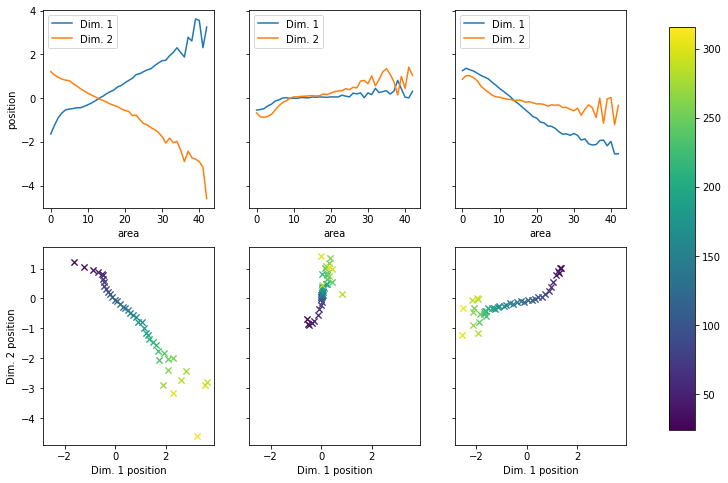
\includegraphics[width=\textwidth]{images/latent_space_traversals/vlae_mnist_morpho_latent_space_values_area.png}
\caption{area}
\end{subfigure}
\hfill
\begin{subfigure}{.48\textwidth}
% include second image
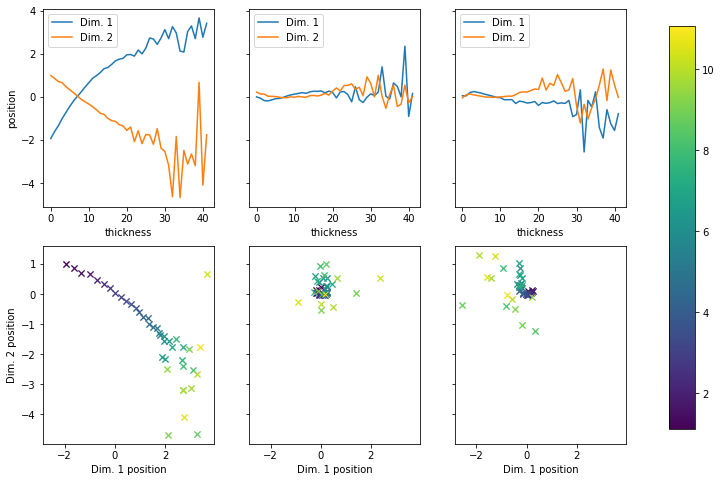
\includegraphics[width=\textwidth]{images/latent_space_traversals/vlae_mnist_morpho_latent_space_values_thickness.png}
\caption{thickness}
\end{subfigure}
\caption{Mean latent space values for \textsc{Mnist}-VLAE when fixing different factors of variation from Morpho-\textsc{Mnist}}
\end{figure}
\end{frame}
\begin{frame}
\begin{figure}
\centering
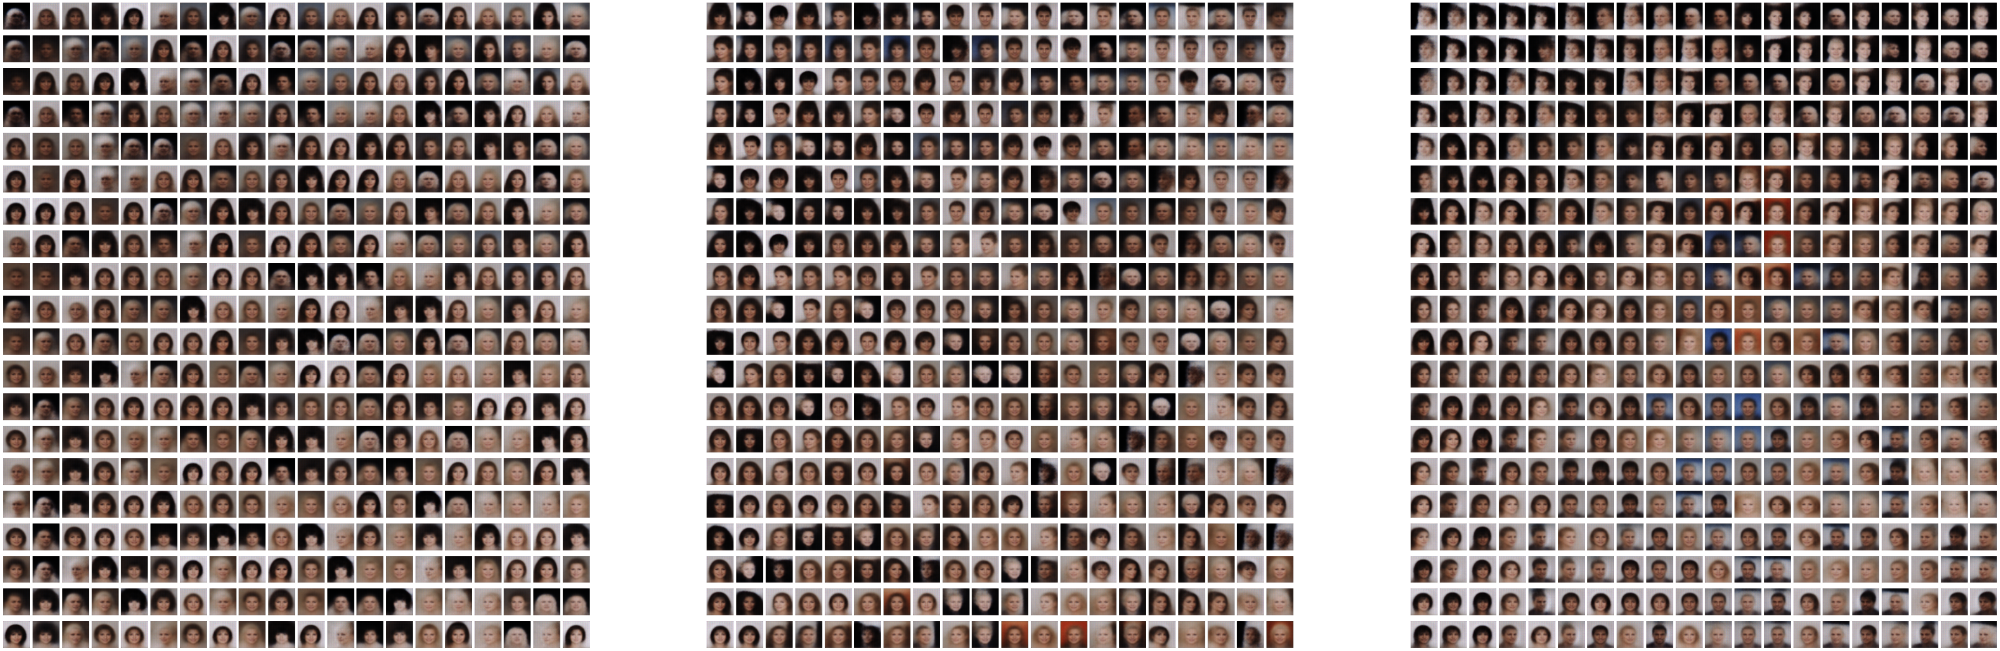
\includegraphics[width=\textwidth]{images/latent_space_traversals/vlae_gan_celeba.png}
\caption[VLAE-GAN on CelebA: Latent Space Exploration]{Latent space exploration of CelebA-VLAE-GAN}
\end{figure}
\end{frame}
\begin{frame}
\begin{figure}
\centering
\begin{subfigure}{.3\textwidth}
% include second image
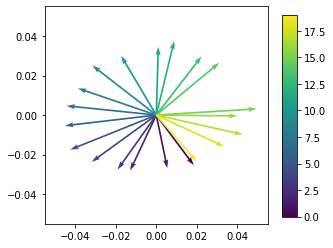
\includegraphics[width=\textwidth]{images/latent_space_traversals/vae_dsprites_orientation_latent_space.png}
\caption{\textit{Ellipse} - only $\frac{1}{2}$ rotation is shown}
\end{subfigure}
\hfill
\begin{subfigure}{.3\textwidth}
% include second image
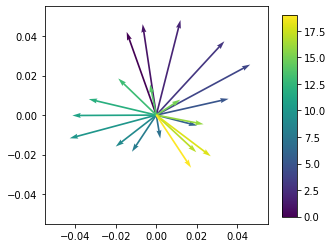
\includegraphics[width=\textwidth]{images/latent_space_traversals/vae_dsprites_orientation_latent_space_heart.png}
\caption{\textit{Heart} - only $\frac{1}{2}$ rotation is shown}
\end{subfigure}
\hfill
\begin{subfigure}{.3\textwidth}
% include second image
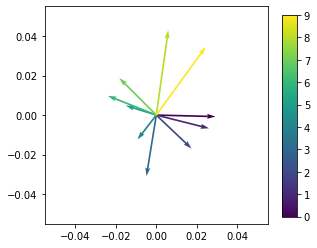
\includegraphics[width=\textwidth]{images/latent_space_traversals/vae_dsprites_orientation_latent_space_square.png}
\caption{\textit{Square} - only $\frac{1}{4}$ rotation is shown}
\end{subfigure}
\caption{PCA-transformed latent space positions of different dsprites shapes with a fixed position, averaged over scales and a 10,000-VAE where only rotation is changed between objects}
\end{figure}
\end{frame}
\begin{frame}
\begin{figure}
\centering
\begin{subfigure}{.48\textwidth}
% include second image
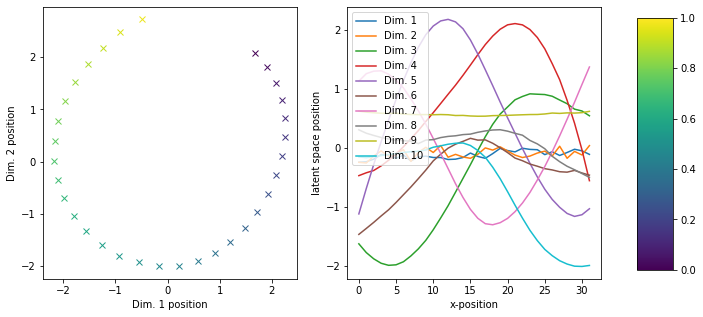
\includegraphics[width=\textwidth]{images/latent_space_traversals/vae_10000_dsprites_latent_space_values_x_position.png}
\caption{Traversal of the reduced latent space for different $x$-positions.}
\label{subfig:vae_dsprites_x_pos_latent_space_route}
\end{subfigure}
\begin{subfigure}{.48\textwidth}
% include second image
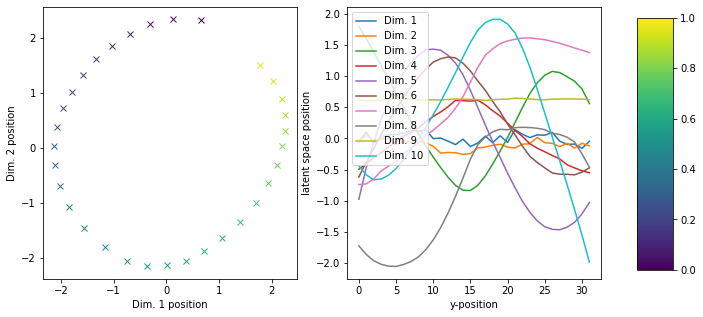
\includegraphics[width=\textwidth]{images/latent_space_traversals/vae_10000_dsprites_latent_space_values_y_position.png}
\caption{Traversal of the reduced latent space for different $y$-positions.}
\label{subfig:vae_dsprites_y_pos_latent_space_route}
\end{subfigure}
\caption[VAE on dsprites: Latent Space Values]{Latent space of 10,000-VAE trained on dsprites. Different values are either for different $x$-positions or for different $y$-position. The other position is fixed to 1.0. It is averaged over all other parameters.}
\end{figure}
\end{frame}
\begin{frame}
\begin{figure}
\centering
\begin{subfigure}{.48\textwidth}
\centering
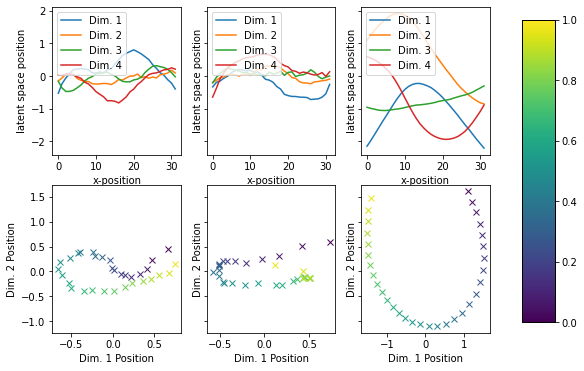
\includegraphics[width=\textwidth]{images/latent_space_traversals/vlae_dsprites_left_latent_space_values.png}
\caption{Varying $x$-position}
\label{subfig:vlae_dsprites_latent_space_values_x}
\end{subfigure}
\hfill
\begin{subfigure}{.48\textwidth}
\centering
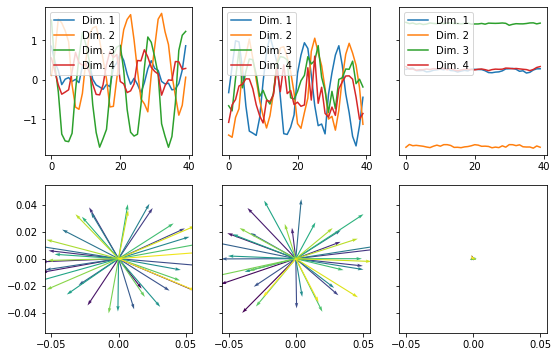
\includegraphics[width=\textwidth]{images/latent_space_traversals/vlae_dsprites_orientation_latent_space_values.png}
\caption{Varying orientation}
\label{subfig:vlae_dsprites_latent_space_values_orientation}
\end{subfigure}
\caption{Values of different dimensions and layers in the VLAE latent space for different factor of variation values, and position in a PCA-reduced latent space. The model was trained on dsprites.}
\end{figure}
\end{frame}
\subsection{Layer Independence - Generated Images}
\begin{frame}
\begin{figure}
\centering
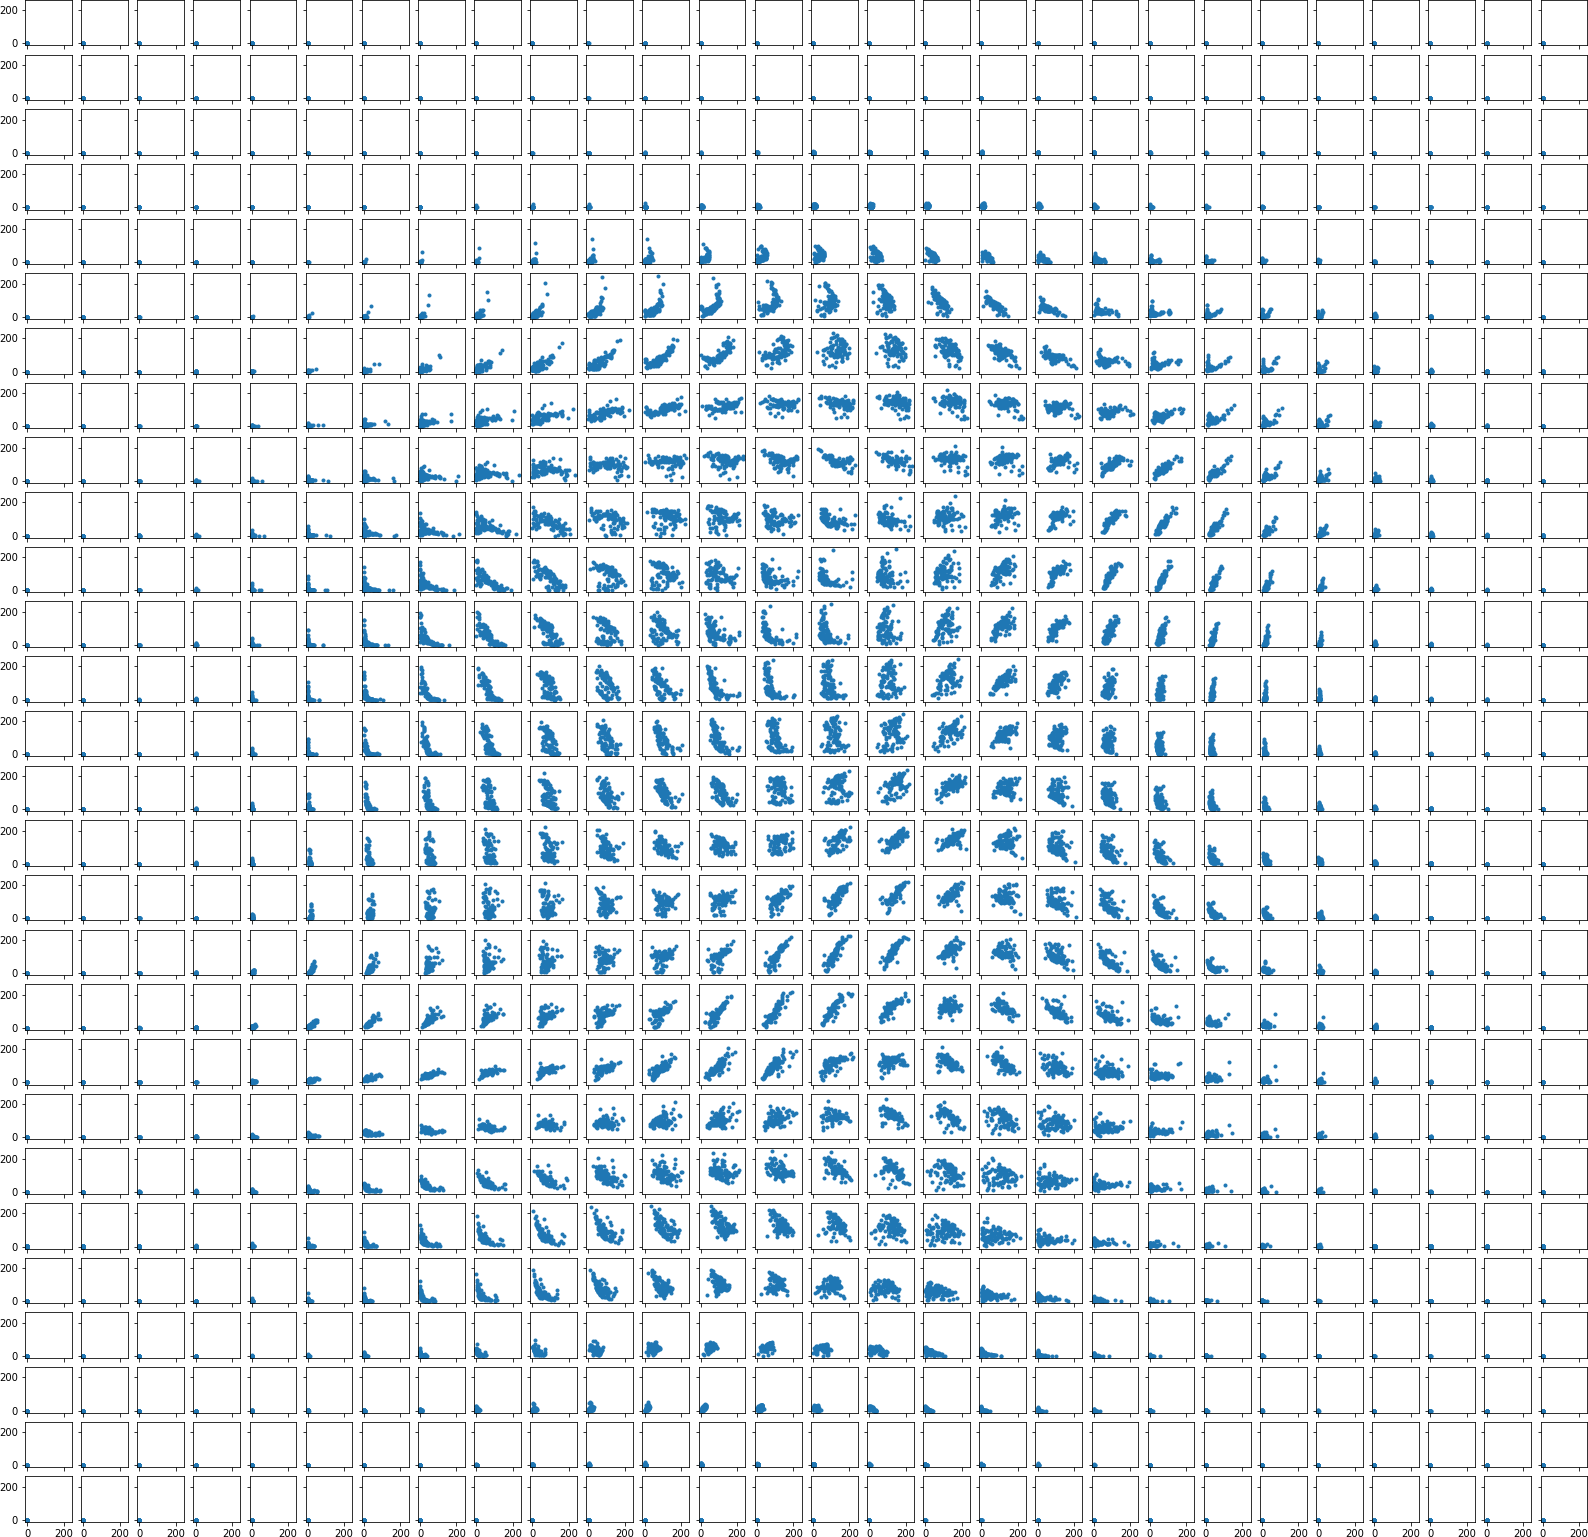
\includegraphics[width=.7\textwidth]{images/notprop/mnist/vlae/ccs_0_1_vlae.png}
\caption{Correlation of pixel intensities when fixing $\bm{z}_1 = \bm{z}_2=\varphi$ for \textsc{Mnist}-VLAE}
\end{figure}
\end{frame}
\begin{frame}
\begin{figure}
\centering
\begin{subfigure}{.3\textwidth}
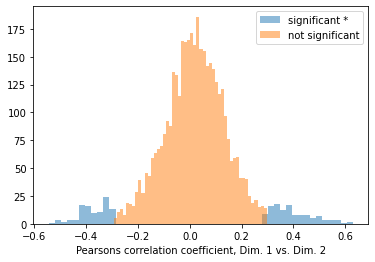
\includegraphics[width=\textwidth]{images/notprop/dsprites/vlae/dim_1_2.png}
\caption{\textsc{Mnist}-VLAE - Layer 1 vs. Layer 2}
\end{subfigure}
\hfill
\begin{subfigure}{.3\textwidth}
\includegraphics[width=\textwidth]{images/notprop/dsprites/vlae/dim_1_3.png}
\caption{\textsc{Mnist}-VLAE - Layer 1 vs. Layer 3}
\end{subfigure}
\hfill
\begin{subfigure}{.3\textwidth}
\includegraphics[width=\textwidth]{images/notprop/dsprites/vlae/dim_2_3.png}
\caption{\textsc{Mnist}-VLAE - Layer 2 vs. Layer 3}
\end{subfigure}
\begin{subfigure}{.3\textwidth}
\includegraphics[width=\textwidth]{images/notprop/dsprites/vlae_gan/dim_1_2.png}
\caption{\textsc{Mnist}-VLAE-GAN - Layer 1 vs. Layer 2}
\end{subfigure}
\hfill
\begin{subfigure}{.3\textwidth}
\includegraphics[width=\textwidth]{images/notprop/dsprites/vlae_gan/dim_1_3.png}
\caption{\textsc{Mnist}-VLAE-GAN - Layer 1 vs. Layer 3}
\end{subfigure}
\hfill
\begin{subfigure}{.3\textwidth}
\includegraphics[width=\textwidth]{images/notprop/dsprites/vlae_gan/dim_2_3.png}
\caption{\textsc{Mnist}-VLAE-GAN - Layer 2 vs. Layer 3}
\end{subfigure}
\caption{Histogram of correlations of pixel-wise intensities when fixing different pairs of dimensions for \textsc{Mnist}-VLAE and \textsc{Mnist}-VLAE-GAN}
\end{figure}
\end{frame}
\subsection{Sparseness in Generative Models}
\begin{frame}
\begin{columns}
\begin{column}{0.3\textwidth}
\begin{figure}
\centering
\includegraphics[height=.8\textheight]{images/sparseness/encoder_fm3_fms.png}
\caption{\textsc{Mnist}-VLAE-factor 3 (active)}
\end{figure}
\end{column}
\begin{column}{0.3\textwidth}
\begin{figure}
\centering
\includegraphics[height=.8\textheight]{images/sparseness/encoder_fm3_fms_inactive.png}
\caption{\textsc{Mnist}-VLAE-factor 3 (inactive) \alert{wrong!}}
\end{figure}
\end{column}
\begin{column}{0.3\textwidth}
\begin{figure}
\centering
\includegraphics[height=.8\textheight]{images/sparseness/encoder_fm3_fms_inactive_correct.png}
\caption{\textsc{Mnist}-VLAE-factor 3 (inactive)}
\end{figure}
\end{column}
\end{columns}
\end{frame}
\begin{frame}
\fontsize{6pt}{7.2}\selectfont
\begin{table}
\centering
\begin{tabularx}{\textwidth}{lXXX}
\toprule
Model                             & mean (SD) - Original & mean (SD) -\linebreak Deactivated & $p$-value \\
\midrule
\textsc{Mnist}-VLAE-factor-1 & 232.759 (8.136)      & \sout{1190.616 (14.710)} 949.648 (12.621)        & $< 0.001$ \\
\textsc{Mnist}-VLAE-factor-2 & 208.107 (6.958)      & \sout{1111.337 (16.326)} 913.353 (11.375)       & $< 0.001$ \\
\textsc{Mnist}-VLAE-factor-3 & 200.258 (6.822)      & \sout{1106.544 (13.942)} 867.842 (11.738)      & $< 0.001$ \\
\bottomrule
\end{tabularx}
\caption[\textsc{Mnist}-VLAEs: Reconstruction Losses]{Reconstruction losses and $p$-values of the comparisons for the original \textsc{Mnist}-VLAE and the versions with deactivated feature maps.}
\end{table}
\end{frame}
\section{Future Work}
\begin{frame}
\begin{itemize}
\item Top-down connections
\item Comparison to IT
\item Sequential data
\end{itemize}
\end{frame}
\section*{References}
\begin{frame}[allowframebreaks]{References}
\printbibliography
\end{frame}
\appendix
\section{Layer Representative Samples}
\begin{frame}[allowframebreaks]
\fontsize{6pt}{7.2}\selectfont
\begin{breakablealgorithm}
\caption{Generating Layer Representative Samples by Averaging Out Other Embedding Layers}\label{alg:layer_representative_samples}
\begin{algorithmic}[1]
\Function{LayerRepresentativeSamples}{numSamples,numApproximations}
\State $j \gets 0$
\State $\mathcal{L}\gets \varnothing$
\While{$i < \text{numSamples}$}
\State $\bm{v} \gets \bm{v} \sim \mathcal{N}(\bm{0}, \bm{I})$\label{line:fixing_v}
\ForAll{$j \in \{1,2,3\}$}
\State $\bm{s}_j \gets$ \Call{LayerRepresentativeSample}{$\bm{v}$, numApproximations, $j$}
\EndFor
\State $\mathcal{L} \gets \mathcal{L} \cup \{\{\bm{s}_1, \bm{s}_2, \bm{s}_3\}\}$

\EndWhile
\State \Return $\mathcal{L}$
\EndFunction

\Function{LayerRepresentativeSample}{fixedDimensionValue, numApproximations, dimensionIndex}
\State $\mathcal{D} \gets \{1,2,3\}$
\State $\alpha \gets \text{fixedDimensionValue}$
\State $\beta \gets (D \setminus \text{dimensionIndex})_1$
\State $\gamma \gets (D \setminus \text{dimensionIndex})_2$
\State $\bm{z}_{\alpha} \gets \bm{a} \sim \mathcal{N}(\bm{0}, \bm{I})$
\State $\mathcal{L}\gets \varnothing$
\State $i \gets 0$
\While{$i < \text{numApproximations}$}
\State $\bm{z}_{\beta}^i \gets \bm{b}_i \sim \mathcal{N}(\bm{0}, \bm{I})$
\State $\bm{z}_{\gamma}^i \gets \bm{c}_i \sim \mathcal{N}(\bm{0}, \bm{I})$
\State $\mathcal{L} \gets \mathcal{L} \cup \{$ \Call{VLAE-Decoder}{$\bm{z}_{\alpha}, \bm{z}_{\beta}^j, \bm{z}_{\gamma}^j$} $\}$
\State $i \gets i + 1$
\EndWhile
\State \Return $\frac{1}{|\mathcal{L}|}\sum_j \mathcal{L}_j$
\EndFunction
\end{algorithmic}
\end{breakablealgorithm}
\end{frame}
\section{Prior vs. Posterior}
\begin{frame}
\begin{figure}
\centering
\begin{subfigure}{0.48\textwidth}
\centering
\includegraphics[width=\textwidth]{images/generated_vs_true/mnist/mnist_vs_models_mean.png}
\end{subfigure}
\hfill
\begin{subfigure}{0.48\textwidth}
\centering
\includegraphics[width=\textwidth]{images/generated_vs_true/mnist/mnist_vs_models_sd.png}
\end{subfigure}
\hfill
\begin{subfigure}{0.48\textwidth}
\centering
\includegraphics[width=\textwidth]{images/generated_vs_true/mnist/mnist_vs_models_skew.png}
\end{subfigure}
\hfill
\begin{subfigure}{0.48\textwidth}
\centering
\includegraphics[width=\textwidth]{images/generated_vs_true/mnist/mnist_vs_models_kurt.png}
\end{subfigure}
\caption{Pixel-wise distributions of different models and moments for the \textsc{Mnist} validation data set - estimated posterior.}
\end{figure}
\end{frame}
\begin{frame}
\begin{figure}
\centering
\begin{subfigure}{0.48\textwidth}
\centering
\includegraphics[width=\textwidth]{images/generated_vs_true/mnist/mnist_vs_models_mean_gauss_post.png}
\end{subfigure}
\hfill
\begin{subfigure}{0.48\textwidth}
\centering
\includegraphics[width=\textwidth]{images/generated_vs_true/mnist/mnist_vs_models_sd_gauss_post.png}
\end{subfigure}
\hfill
\begin{subfigure}{0.48\textwidth}
\centering
\includegraphics[width=\textwidth]{images/generated_vs_true/mnist/mnist_vs_models_skew_gauss_post.png}
\end{subfigure}
\hfill
\begin{subfigure}{0.48\textwidth}
\centering
\includegraphics[width=\textwidth]{images/generated_vs_true/mnist/mnist_vs_models_kurt_gauss_post.png}
\end{subfigure}
\caption{Pixel-wise distributions of different models and moments for the \textsc{Mnist} validation data set - Gaussian prior.}
\end{figure}
\end{frame}
\end{document}